%%%%%%%%%%%%%%%%%%%%%%%%%%%%%%%%%_TEMPLATE_PACKAGES_%%%%%%%%%%%%%%%%%%%%%%%%%%%%%%%%%
\documentclass[
	a4paper,
	pagesize,
	pdftex,
	12pt,
	% twoside,    % + BCOR darunter: für doppelseitigen Druck aktivieren, sonst beide deaktivieren
	% BCOR=5mm,   % Dicke der Bindung berücksichtigen (Copyshop fragen, wie viel das ist)
	english,
	fleqn,
	final,
	]{scrartcl}
    
% PACKAGES FOR THE INSTITUTSVORLAGE
\usepackage[utf8]{inputenc}
\usepackage[english]{babel}
\usepackage[unicode=true,hidelinks]{hyperref} % label, references, websites and crosslinks in PDF
\usepackage{setspace} % für Elemente der Titelseite
\usepackage{tikz} % für Elemente der Titelseite
\usepackage{tabularx} % für Elemente der Titelseite
\usepackage[draft=false,babel,tracking=true,kerning=true,spacing=true,verbose=silent]{microtype} % optischer Randausgleich
\microtypesetup{nopatch={footnote}} % disable footnote microtype warning
% PACKAGES FOR USING THIS PREBUILD STUCTURE
\usepackage{csquotes}   % better quote style for biblatex
\usepackage{graphicx}
%%%%%%%%%%%%%%%%%%%%%%%%%%%%%%%%%_YOUR_PACKAGES_%%%%%%%%%%%%%%%%%%%%%%%%%%%%%%%%%
% UTILITY PACKAGES
\usepackage{cite}
\usepackage{comment} % enables block comments via \begin{comment} ... \end{comment} environment
\usepackage{amsthm} % for definitions, lemmas, etc. - also for defining your own stuff, eg below:
    %\theoremstyle{definition}  % defines a new theorem called definition
    %\newtheorem{definition}{Definition}[section]   % definition setup and call
% IMAGE PACKAGES
\usepackage{wrapfig}    % create figures with wrapped text around it
\usepackage{caption}    % better captions for figures
\usepackage{subcaption} % captions for subfigures
% PRESENTATION PACKAGES
\usepackage{booktabs} % for professional tables
\usepackage{longtable} % for tables over multiple pages
\usepackage{pdflscape} % enables landscape mode for multiple pages in PDF (with longtable)
\usepackage{afterpage} % clears current page by flushing all floats
%%%%%%%%%%%%%%%%%%%%%%%%%%%%%%%%%%%_TITLE_PAGE_%%%%%%%%%%%%%%%%%%%%%%%%%%%%%%%%%%%
\begin{document}

% Beispielhafte Nutzung der Vorlage für die Titelseite (bitte anpassen):
% LaTeX-Vorlage für die Titelseite und Selbständigkeitserklärung einer Abschlussarbeit
% basierend auf der vorigen Institutsvorlage des Instituts für Informatik
% sowie der Vorlage für Promotionsarbeiten.
%%%%%%%%%%%%%%%%%%%%%%%%%%%%%%%%%%%%%%%%%%%%%%%%%%%%%%%%%%%%%%%%%%%%%%%%%%%%%%%%%%%%
% CHANGELOG
% 2014-06-12 Dennis Schneider <dschneid@informatik.hu-berlin.de> (Erweiterung)
% 2023-02-28 Anna Göing <goeingan@informatik.hu-berlin.de> (Strukturhilfe + Packageupdate) 
% 2023-07-14 Florian Willich <florian.willich@informatik.hu-berlin.de> (Formal Revision, Abstract, Package Revision)
%%%%%%%%%%%%%%%%%%%%%%%%%%%%%%%%%%%%%%%%%%%%%%%%%%%%%%%%%%%%%%%%%%%%%%%%%%%%%%%%%%%%
% gepunktete Linie unter Objekt:
\newcommand{\TitelPunkte}[1]{%
  \tikz[baseline=(todotted.base)]{
    \node[inner sep=1pt,outer sep=0pt] (todotted) {#1};
    \draw[dotted] (todotted.south west) -- (todotted.south east);
  }%
}%
% gepunktete Linie mit gegebener Länge:
\newcommand{\TitelPunktLinie}[1]{\TitelPunkte{\makebox[#1][l]{}}}
\makeatletter
%
\newcommand*{\@titelTitel}{Titel der Arbeit}
\newcommand{\titel}[1]{\renewcommand*{\@titelTitel}{#1}} % Titel der Arbeit
\newcommand*{\@titelArbeit}{Arbeitstyp}
\newcommand{\typ}[1]{\renewcommand*{\@titelArbeit}{#1}} % Typ der Arbeit
\newcommand*{\@titelGrad}{akademischer Grad}
\newcommand{\grad}[1]{\renewcommand*{\@titelGrad}{#1}} % Akademischer Grad
\newcommand*{\@titelAutor}{Autor}
\newcommand{\autor}[1]{\renewcommand*{\@titelAutor}{#1}} % Autor der Arbeit
\newcommand*{\@titelGeburtsdatum}{\TitelPunktLinie{2cm}}
\newcommand{\gebdatum}[1]{\renewcommand*{\@titelGeburtsdatum}{#1}} % Geburtsdatum des Autors
\newcommand*{\@titelGeburtsort}{\TitelPunktLinie{5cm}}
\newcommand{\gebort}[1]{\renewcommand*{\@titelGeburtsort}{#1}} % Geburtsort des Autors
\newcommand*{\@titelGutachterA}{\TitelPunktLinie{5cm}}
\newcommand*{\@titelGutachterB}{\TitelPunktLinie{5cm}}
\newcommand{\gutachter}[2]{\renewcommand*{\@titelGutachterA}{#1}\renewcommand*{\@titelGutachterB}{#2}} % Erst- und Zweitgutachter
\newcommand*{\@titelEinreichungsdatum}{\TitelPunktLinie{3cm}} % Datum der Einreichung, wird nicht vom Studenten ausgefüllt
\newcommand*{\@titelVerteidigungsdatum}{} % Verteidigungstext, wird nicht vom Studenten ausgefüllt
\newcommand{\mitverteidigung}{\renewcommand*{\@titelVerteidigungsdatum}{verteidigt am: \,\,\TitelPunktLinie{3cm}}} % Verteidigungsplatzhalter erzeugen
\newcommand*{\@wastwoside}{}
%%
% Titelseite erzeugen:
\newcommand{\makeTitel}{%
	% Speichere, ob doppelseitiges Layout gewählt wurde:
\if@twoside%
	\renewcommand*{\@wastwoside}{twoside}
\else
	\renewcommand*{\@wastwoside}{twoside=false}
\fi
	\KOMAoptions{twoside = false}% Erzwinge einseitiges Layout (erzeugt eine Warnung)
%
	\begin{titlepage}
		% Ändern der Einrückungen
		\newlength{\parindentbak} \setlength{\parindentbak}{\parindent}
		\newlength{\parskipbak} \setlength{\parskipbak}{\parskip}
		\setlength{\parindent}{0pt}
		\setlength{\parskip}{\baselineskip}
		\thispagestyle{empty}
		%
		\begin{minipage}[c][3cm][c]{12cm}
			\textsc{%
				% optischer Randausgleich per Hand:
				\hspace{-0.4mm}\textls*[68]{\Large Humboldt-Universität zu Berlin}\\
				\normalsize \textls*[45]{
					Mathematisch-Naturwissenschaftliche Fakultät\\
					Institut für Informatik
				}
			}
		\end{minipage}
\hfill
		\vfill
		%
		\vspace*{\fill}
		\begin{center}
		\begin{doublespace}
			\vspace{\baselineskip}
			{\LARGE \textbf{\@titelTitel}}\\
			%\vspace{1\baselineskip}
			{\Large
			\@titelArbeit\\
				zur Erlangung des akademischen Grades\\
				\@titelGrad
				\vspace{\baselineskip}
				}
		\end{doublespace}
		\end{center}

		\vfill
\newcolumntype{L}{>{\raggedright\arraybackslash}X}
		{\large \raggedleft
			\begin{tabularx}{\textwidth}{l@{\,\,\raggedright~}L} % verbreiterter Abstand zwischen Feldern wurde gewünscht
				eingereicht von: & \@titelAutor\\
				geboren am: & {\@titelGeburtsdatum}\\
				geboren in: & \@titelGeburtsort
				\vspace{0.5\baselineskip}\\
				Gutachter/innen: & \@titelGutachterA \\
					& \@titelGutachterB
				\vspace{0.5\baselineskip}\\
				eingereicht am: & \@titelEinreichungsdatum \hfill \@titelVerteidigungsdatum
			\end{tabularx}}
			\vspace{-1\baselineskip}\\\phantom{x} % Übler Hack, um eine Warnung wg. einer zu leeren hbox zu verhindern
		% Wiederherstellen der Einrückung
		\setlength{\parindent}{\parindentbak}
		\setlength{\parskip}{\parskipbak}
	\end{titlepage}
%
	% Aufräumen:
	\let\@titelTitel\undefined
	\let\titel\undefined
	\let\@titelArbeit\undefined
	\let\typ\undefined
	\let\@titelGrad\undefined
	\let\grad\undefined
	\let\@titelAutor\undefined
	\let\autor\undefined
	\let\@titelGeburtsdatum\undefined
	\let\gebdatum\undefined
	\let\@titelGeburtsort\undefined
	\let\gebort\undefined
	\let\@titelGutachterA\undefined
	\let\@titelGutachterB\undefined
	\let\gutachter\undefined
	\let\@titelEinreichungsdatum\undefined
	\let\einreichungsdatum\undefined
	\let\@titelVerteidigungsdatum\undefined
	\let\verteidigungsdatum\undefined
%
	\KOMAoptions{\@wastwoside}% Stelle alten Modus (ein-/doppelseitig) wieder her
	\let\@wastwoside\undefined
	\cleardoublepage % ganzes Blatt für die Titelseite
}
% Als Allerallerletztes kommt Selbständigkeitserklärung:
\newcommand{\selbstaendigkeitserklaerung}[1]{%
	%\cleardoublepage% Wieder auf eine eigene Doppelseite
	{\parindent0cm
		\subsection*{Selbständigkeitserklärung}
		Ich erkläre hiermit, dass ich die vorliegende Arbeit selbständig verfasst
		und noch nicht für andere Prüfungen eingereicht habe.
		Sämtliche Quellen einschließlich Internetquellen, die unverändert oder
		abgewandelt wiedergegeben werden, insbesondere Quellen für Texte, Grafiken,
		Tabellen und Bilder, sind als solche kenntlich gemacht. Mir ist bekannt,
		dass bei Verstößen gegen diese Grundsätze ein Verfahren wegen
		Täuschungsversuchs bzw. Täuschung eingeleitet wird.
		\vspace{3\baselineskip}

		{\raggedright Berlin, den #1 \hfill \TitelPunktLinie{8cm}\\}
	}
}%
\makeatother


\titel{Likertshift - an input device for monitoring Travel Experience while cycling} % Titel der Arbeit
\typ{Bachelorarbeit} % Typ der Arbeit:  Diplomarbeit, Masterarbeit, Bachelorarbeit
\grad{Bachelor of Science (B. Sc.)} % erreichter Akademischer Grad
    % z.B.: Master of Science (M. Sc.), Master of Education (M. Ed.), Bachelor of Science (B. Sc.), Bachelor of Arts (B. A.)
\autor{Max Schlecht} % Autor der Arbeit, mit Vor- und Nachname
\gebdatum{08.06.2000} % Geburtsdatum des Autors
\gebort{Berlin} % Geburtsort des Autors
\gutachter{Prof. Dr. Thomas Kosch}{Prof. Dr. Andrii Matviienko} % Erst- und Zweitgutachter der Arbeit
\mitverteidigung % entfernen, falls keine Verteidigung erfolgt
\makeTitel

\begin{abstract}
    \subsubsection*{Abstract}
    This work explores creating an improved method for recording real-time ground truth data on cyclists' subjective experiences.
    It presents the design process of a physical prototype, resembling a standard bicycle twist gearshift, which enables cyclists to provide ratings on a Likert scale without interrupting their cycling or compromising their safety.
    A field study was conducted to evaluate the prototype against other state-of-the-art methods.
    Results showed that participants strongly preferred using our prototype, highlighting its ease of use, intuitive handling, and lack of concerns regarding social acceptance or additional time requirements compared to other methods.
    Additionally, an evaluation of the recorded travel satisfaction data confirmed that the data collected using the prototype was of comparable or superior quality to that collected using existing methods.
    This research paves the way for larger field studies by providing a better method to either directly record cyclists' subjective experiences or the necessary ground truth data to infer their emotions from additional contextual or sensory data.
\end{abstract}

\newpage

%%%%%%%%%%%%%%%%%%%%%%%%%%%%%%%%_TABLE_OF_CONTENTS_%%%%%%%%%%%%%%%%%%%%%%%%%%%%%%%%
\pagenumbering{gobble}  % page numbers invisible for TOC and filler pages
\tableofcontents
\cleardoublepage    % deactivate for one-sided printing
%\newpage           % activate for one-sided printing
%%%%%%%%%%%%%%%%%%%%%%%%%%%%%%%%%%%%%_CHAPTERS_%%%%%%%%%%%%%%%%%%%%%%%%%%%%%%%%%%%%%
\pagenumbering{arabic}  % start regular page numbers from here
% insert and call your designated chapters here from chapters/... folder

\newpage\section{Motivation}\label{sec:motivation}

Recent works in the HCI space have been exploring detecting drivers' emotions while operating vehicles and understanding their effects.
Many of them specifically focus on negative emotional extremes, such as anger and sadness \cite{driver_emotion_recognition_survey}, as these not only lead to an increased number of driving errors \cite{dont_cry_while_youre_driving} but can also encourage more risky behaviors like speeding \cite{negative_or_positive,frequency_determinants_and_consequences}.

Consequently, there is also a growing interest in developing affective user interfaces that can utilize said emotions to enhance user satisfaction and traffic safety.
Examples of such affective user interfaces include route planners that do not only offer the fastest routes but also ones that evoke more positive emotions in drivers \cite{what_if_your_car_would_care}, voice assistants that adapt their tone empathically \cite{affective_automotive_user_interfaces,emotional_adaptive_vehicle_user_interfaces}, or even systems that prevent operation altogether if the driver is deemed incapable of operating the vehicle \cite{affective_automotive_user_interfaces}.
\citetext{towards_empathetic_car_interfaces}{Zepf et al.} also investigated what situations during driving trigger certain emotions and categorized them, recommending measures to mitigate those that negatively impact driving performance.

Many of these studies, particularly real-world ones, rely on real-time audio-based self-reporting to obtain their results \cite{towards_empathetic_car_interfaces,vemotion,frequency_determinants_and_consequences}.
In an automotive context, this method is practical, as microphones can easily be mounted inside vehicles, which provide an environment with a generally well-predictable noise floor.
Automatic voice processing can then be used to obtain the desired data \cite{vemotion}.

\bigbreak\noindent
While most of this research has focused on travel by car, the ongoing shift toward sustainable transportation, especially in urban areas, has generated significant interest in expanding it to other modes of individual transportation, most notably cycling.

Similar to automotive contexts, data on \CSE can be used to improve traffic safety, infrastructure planning \cite{the_influence_of_noise,emotion_sensing_for_ebike_safety}, as well as the overall experience and satisfaction of cyclists, thereby engaging more people in a more sustainable and healthy mode of transportation \cite{exploring_the_casual_effects,health_benefits_of_cycling,happy_or_scared}.

Personalized route planning, for example, gains even more significance in the context of cycling, as there is not only a larger variance in road conditions and types of bicycle paths but also in cyclists' preferences concerning them.
For instance, some cyclists may prefer riding only on well-maintained, flat asphalt roads, while others might actually enjoy more rugged, off-road paths.
To properly detect and differentiate between triggers (e.g., weather, road condition, traffic) affecting the subjective experience of cyclists while riding, subjective real-time ratings must be consolidated with accurate time and location data, as well as external contextual data \cite{cycling_subjective_experience}.

Multiple recent large reviews have found that existing studies predominantly rely on retrospective surveys and interviews as methods to evaluate \CSE \cite{cycling_subjective_experience,physiological_measures_of_bicyclists,methods_used_to_capture}.
\citetext{cycling_subjective_experience}{Zhang et al.} also claim that recently, there has been a growing interest in utilizing more mobile methods capable of capturing real-time data during cycling.

Methods that try to predict cyclists' emotions from contextual information such as driving behavior, weather, or traffic could also provide such real-time data.
\citetext{vemotion}{Bethge et al.} demonstrated that emotion recognition models based on contextual data can even outperform traditional techniques like facial expression recognition.
However, creating mathematical models or training machine learning models like this still requires obtaining ground-truth data from study participants in the first place, further underlining the need for developing better self-reporting methods \cite{detecting_stress,vemotion,happy_or_scared,evaluation_models_for_cyclists_perception}.

\bigbreak\noindent
We argue that data obtained from retrospective methods often lacks the required detail \cite{cycling_subjective_experience}, while live recording methods, namely mobile audio self-reporting, have been directly adopted from automotive research on the subject but are unsuitable for cycling due to social and environmental factors.
Thus, to advance this field and enable researchers to collect real-time ground-truth data on \CSE more effectively, we want to develop a new method using an electromechanical device that allows cyclists to self-report values on a simple one-dimensional scale.

We start by reviewing related work on existing real-time methods for recording cyclists' subjective experiences and digital control devices for cycling. From this, we derive a set of design requirements that guide the development of our prototype. Finally, we conduct a field study comparing our prototype to existing real-time recording methods, evaluate its performance, and discuss our results and how they could affect future research in the field.

\newpage\section{Related Work}\label{sec:related_work}


\cite{cycling_subjective_experience}

\subsection{Digital Control Devices for Bicycles}

\cite{brotate_and_tribike}
\subsection{Methods for Recording \CSE}

\subsection{Research Questions}

\newpage\section{Prototype Design}\label{sec:prototype_design}

\subsection{Design Requirements}

To streamline the design of our prototype and to ensure its usefulness to other researchers in future work, we established the following design requirements:

\begin{enumerate}[label=\textsf{DRQ\arabic*}, left=1em .. 4.5em]
    \item \textbf{Intuitive}\label{drq:intuitive}\\
        Controlling the prototype device should be intuitive to the user.

    \item \textbf{Robust}\label{drq:robust} \\
        Using the prototype device should require minimal user intervention and maintenance. Users should not be able to easily break the device, and it should withstand external influences such as humidity and temperature variations.

    \item \textbf{Safe}\label{drq:safe}\\
        The prototype device should not compromise the user's safety.

    \item \textbf{Affordable}\label{drq:affordable}\\
        The total cost of all required components should not exceed \euro25.00.

    \item \textbf{Easy to Reproduce}\label{drq:easy_to_reproduce}\\
        The prototype device should be able to be manufactured and assembled using standard tools commonly available in most research laboratories.
\end{enumerate}

\noindent
In \autoref{subsec:discussion_design_requirements} we analyze how well our final prototype device meets these requirements based on the results gathered from our field study.

\subsection{Mechanical Design}

\subsubsection{Initial Design Decisions}

\subsubsection*{Continuous or Discrete Scale}

As discussed in \autoref{sec:motivation}, our prototype device should enable users to communicate their Travel Experience on a simple one-dimensional scale.
We need to decide whether this scale should be continuous or consist of discrete steps.

Theoretically, we would be able to capture more precise data with a continuous scale than with a discrete one.
However, since our use case is recording Travel Experience data - which is highly subjective - recorded values will vary significantly between different users.
So to obtain meaningful results, any recorded Travel Experience data must be averaged across a reasonably large pool of different users.
Therefore, a continuous input scale would not provide a substantial benefit for our specific use case.

This decision also directly influences the electromechanical design of the device.
Choosing to design a continuous scale would force us to either use a variable resistor (potentiometer) or a high resolution digital encoder.
In contrast, working with discrete steps would suggest the use of a rotary switch or multiple mechanical buttons.

Due to the missing benefit of a continuous scale and our previous decision to use a custom-built mechanism, we decided on a discrete scale, because we think this will be easier to implement using our chosen methods.

\cite{gesturing_on_the_handlebars} \cite{no_need_to_stop} \cite{text_me_if_you_can} \cite{brotate_and_tribike}

\begin{itemize}
    \item potentiometers vs. rotary switches vs. buttons
    \item brotate and tribike \cite{brotate_and_tribike}
    \item advantages/disadvantages of using our own hardware design (cost, reliability, availability, obsolete components)
\end{itemize}

\subsection{Electrical Design and Firmware}

\begin{itemize}
    \item BLE
    \item MCU choice (softdevices conformity)
    \item battery runtime analysis
\end{itemize}

\subsection{Frontend Design}

\begin{itemize}
    \item reusability
    \item BLE interfacing (communication "protocol")
    \item language/framework choice?
    \item UI design?
\end{itemize}

\newpage\section{Study Design}\label{sec:study_design}

We decided to evaluate our prototype in a semi-naturalistic field-study, comparing it against similar methods, capable of recording \CSE for individual segments of a larger route.
This section describes how we went about designing this study.

\subsection{Recording Methods}\label{subsec:recording_methods}

Our method using the “LikertShift” device works by recording its currently selected value, whenever we receive a new GPS location.
Thus, a selected value remains valid until the users selects a new one, and we receive their next GPS location, so a new rating gets recorded whenever they notice a change in their subjective experience and remains valid, onwards from that point in time, until they adjust the rating again.
This allows users to choose a rating frequency they consider appropriate by themselves.

We selected two methods from our survey of the related work we regard as suitable to compare against our method and adjusted them, to allow for a fair comparison.
The first one, referred to as “Audio Recording” from now on, is taken from the work of \citetext{evaluation_models_for_cyclists_perception}{Yamanaka et al.}, who captured audio data while cycling and required participants to rate pre-defined route-segments using multiple measures on scales from 1 to 5.
We adjusted it to only used one measure and also let participants perform ratings on arbitrary route segments, in contrast to pre-defined ones.
The second method, referred to as “Mapping” is the one proposed by \citetext{using_mental_mapping}{Manton et al.}, who let participants color code segments of a previously driven route, based on their risk assessment.
In our study, we provided participants with a printed map, picturing the route they drove and let them divide it into multiple segments themselves, assigning a numerical rating to each segment, instead of color coding it.

\subsubsection*{Choosing a Measure}

We had to take great care to select a suitable measure, so we could compare the data collected by different participants and the different methods against each other.
This is inherently difficult, as cyclists' subjective experiences are arguably very subjective and will thus vary drastically from participant to participant.

As mentioned in the introduction to \autoref{sec:related_work}, most works rely on risk/safety and stress/comfort measures to quantify \CSE.
The advantage of using risk/safety would be its independence from many external factors and high dependence on the chosen route.
Constructing a route with highly varying risk factors would be comparatively easy, but deliberately placing participants in high-risk environments would be extremely unethical, which led us to quickly dismiss that approach.
Letting participants rate their comfort level or travel satisfaction comes with its own set of challenges though.
Overall comfort level depends on a lot of actors, such as participants initial mood, their experience in riding a bicycle, but also external factors such as weather, traffic, or surrounding scenery of the route.
To be able to properly compare our recorded datasets against each other, we needed to find a way to eliminate as many of these factors as possible.

As findings by \citetext{thinking_aloud_on_the_road}{McIlroy et al.} revealed the high impact of road surface quality on cyclists overall comfort and satisfaction with their travel, we decided to limit our measure to this, using the metric of “Travel satisfaction, based on the road” as the \CSE measure that participants have to use to rate segments of the route.
We carefully explained this metric to each participant before conducting the study, instructing them on what should (road condition, road type, available space, slope of the road, etc.) and should not (general mood, current traffic situation, route scenery, etc.) affect their ratings.
Ratings were to be performed on a Likert scale from 1 to 5, denoting high dissatisfaction and high satisfaction, respectively.
This measure should exert a similar mental demand on participants, as they still need to feel out their comfort level, while increasing data quality, allowing us to perform quantitative comparisons of the different methods used.
\subsection{Route Selection}

If each participant was to evaluate all three methods after each other on the same route, we would expect to see an increase in accuracy for subsequent route traversals, as by that point the route is already known.
Thus, we constructed three different routes and balanced route orders, method orders as well as the number of routes per method in our study.
We chose each route to take $\sim\SI{10}{min}$ to complete for an average cyclist and ensured it contained a multitude of different road types and crossings.
As we wanted to conduct the study in a single session per participant, at our university campus, we were limited by the available traffic infrastructure in the immediate vicinity and also had to put all start and endpoints in the approximate same location.

\begin{table}[!htb]
    \footnotesize
    \centering
    \begin{tabular}{c|c|ccccc|c}
        \multirow{2}{*}{Name} & \multirow{2}{2.4em}{Total\newline} & \multicolumn{5}{c|}{Road Type} & \multirow{2}{4.7em}{Number of\newline}\\
        \cline{3-7}
        &&&&&&&\\[-1em]
        & Length & Road & Bike Path & Mixed Path & Pedestrian Way & Other & Crossings\\[0.15em]
        \hline
        &&&&&&&\\[-0.8em]
        North & \SI{2589}{m} &  \SI{191}{m} & \SI{480}{m} & \SI{1135}{m} & \SI{359}{m} & \SI{424}{m} & 13\\[0.3em]
        East  & \SI{2007}{m} &  \SI{853}{m} & \SI{465}{m} &  \SI{173}{m} & \SI{181}{m} & \SI{335}{m} & 9\\[0.3em]
        South & \SI{2289}{m} & \SI{1152}{m} & \SI{677}{m} &  \SI{116}{m} &  \SI{47}{m} & \SI{297}{m} & 9\\
    \end{tabular}
    \caption{Overview of the study routes}
    \label{table:routes_overview}
\end{table}

\noindent
\autoref{table:routes_overview} shows the total lengths of the routes, as well as an overview of the different road types and number of crossings per route.
Each route is named according to the direction it starts towards.
The study was conducted at the Campus Adlershof\footnoteurl{https://www.hu-berlin.de/en/about/campus/adlershof} of the Humboldt University of Berlin, located in a mixed-use area outside the city center.
Notably, the roads participants had to drive on were mostly side-roads with very little traffic and therefore received a more positive rating than one might expect.
We also opted to use existing cycling infrastructure wherever possible, only evading to drive on the road when no such infrastructure was available.
Furthermore, mixed-paths refer to areas mainly intended to be used by pedestrians that are spacious enough to allow for cycling at low speeds.

\begin{figure}[!htb]
    \centering
    \begin{minipage}{.5\textwidth}
        \centering
        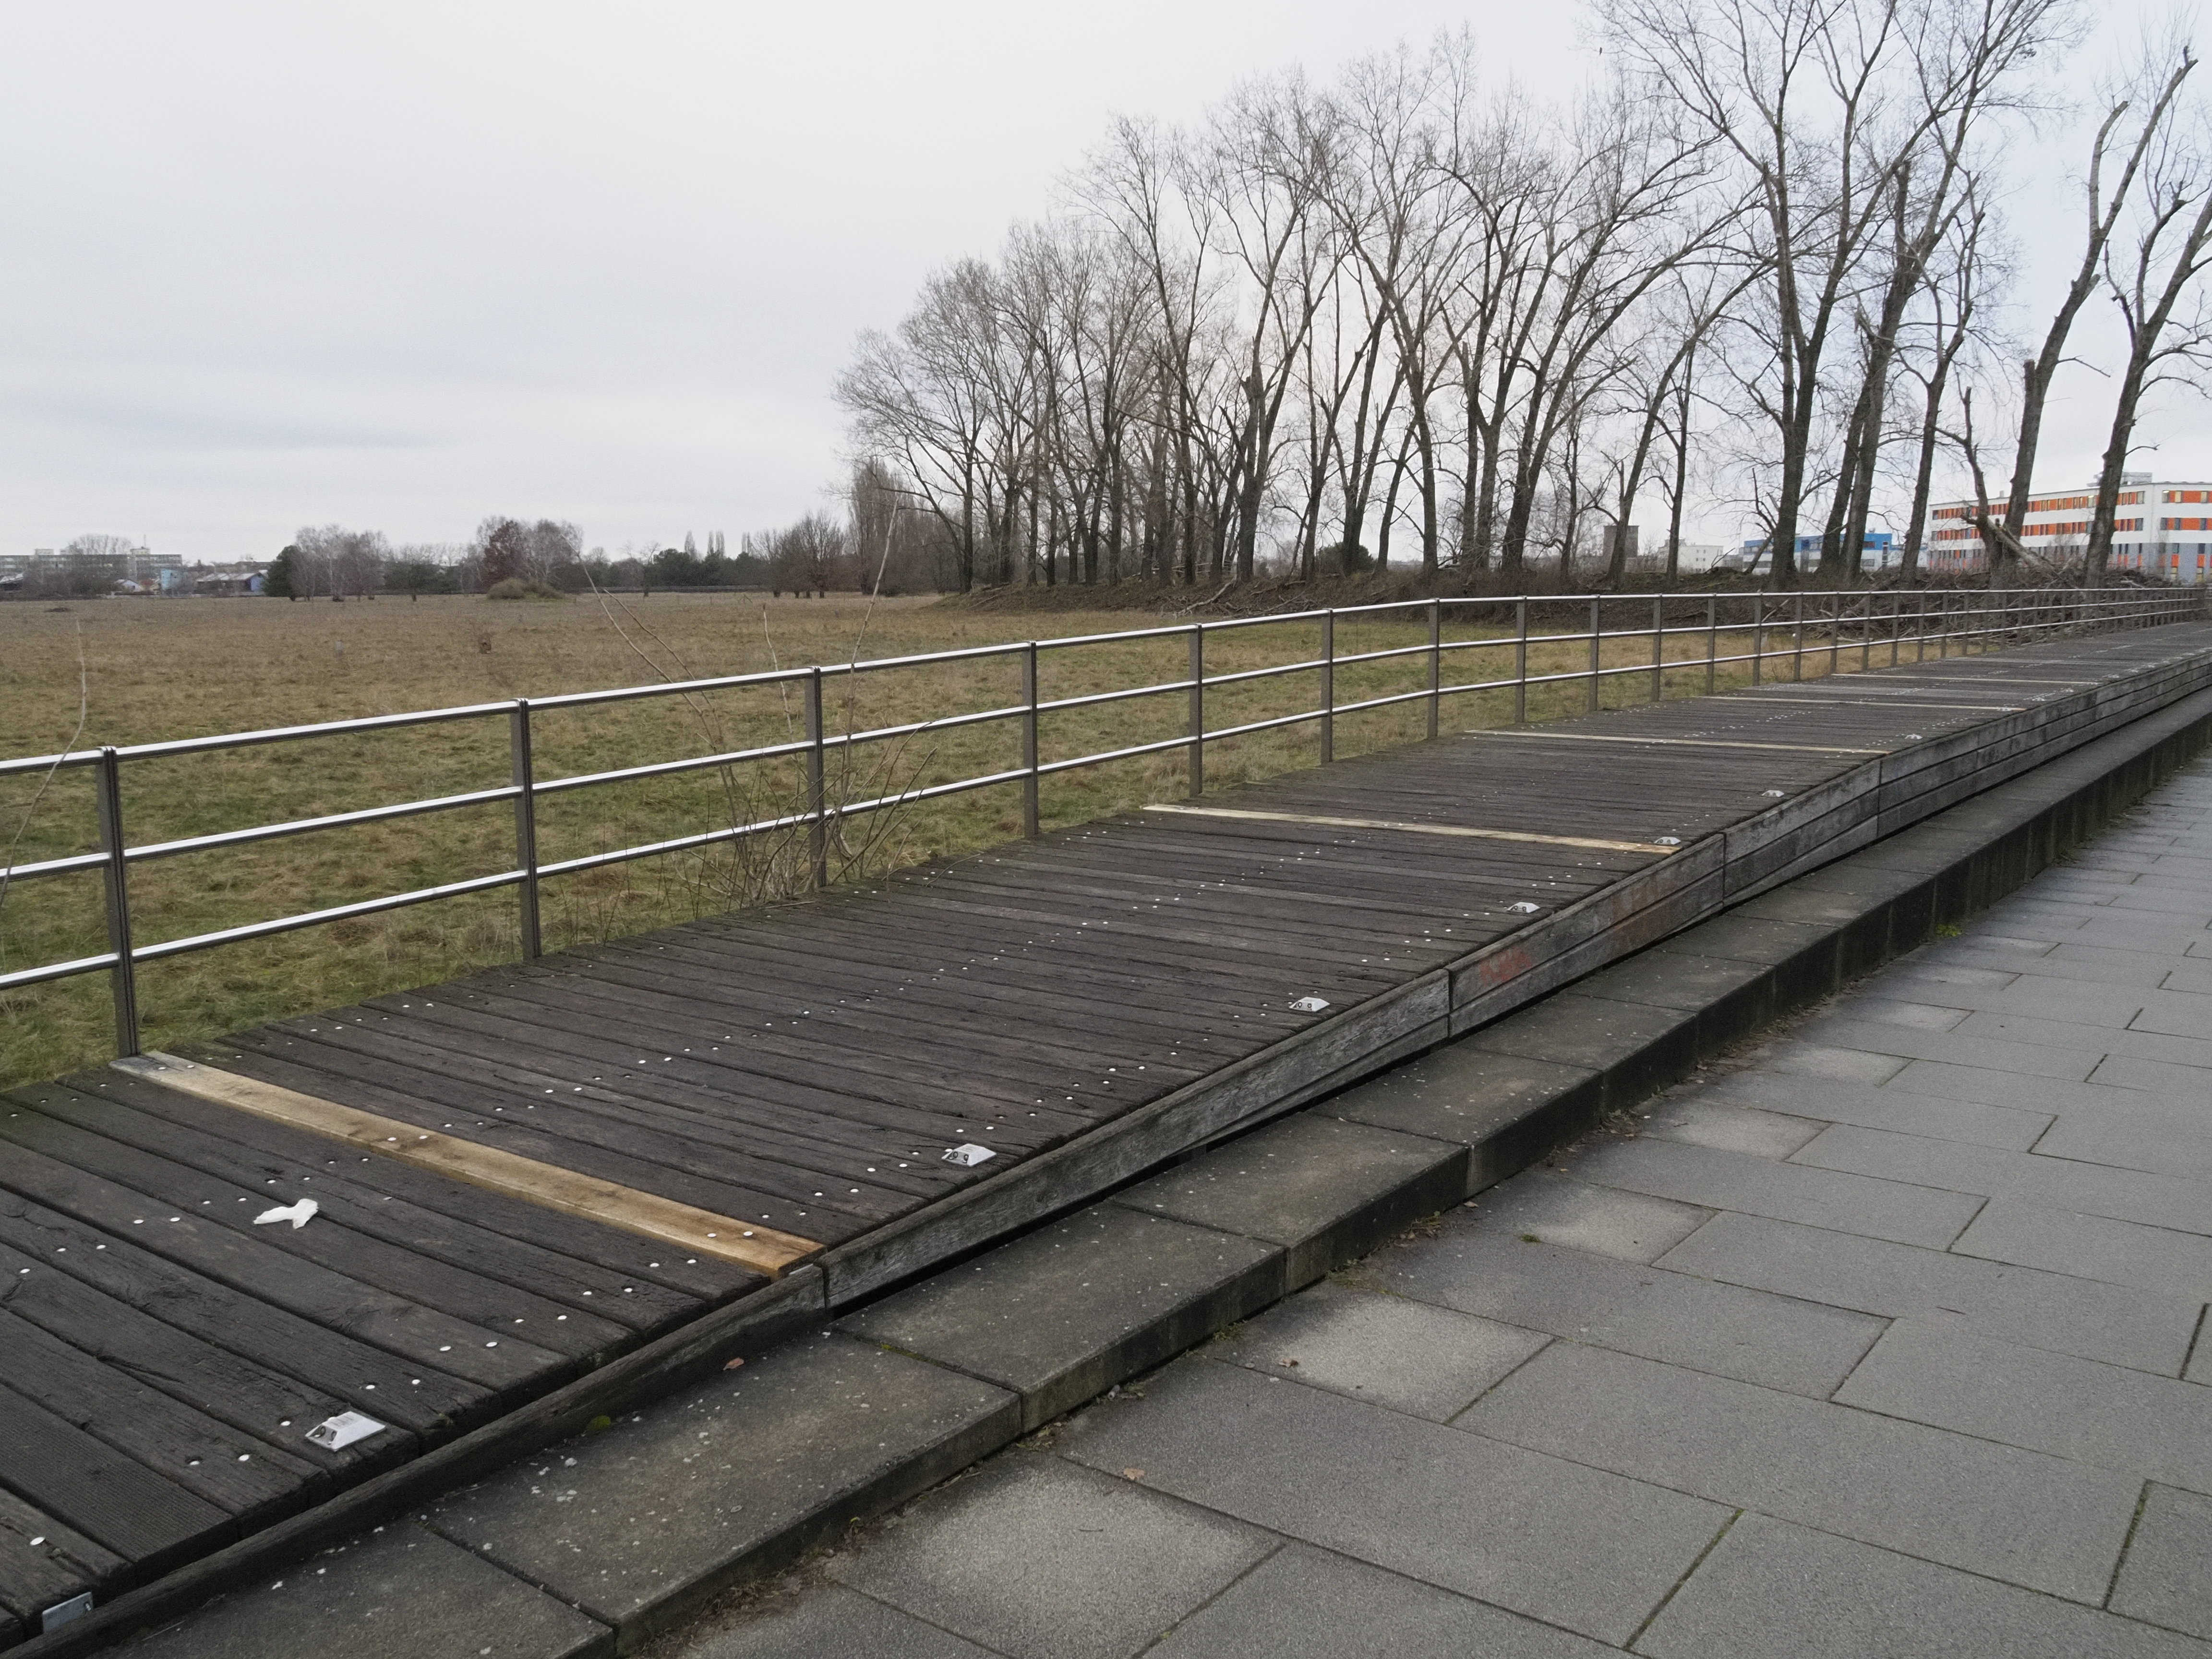
\includegraphics[width=.9333\linewidth]{images/wood_planks_path.jpg}
        \caption{Elevated path (wood planks)}
        \label{fig:wood_planks}
    \end{minipage}%
    \begin{minipage}{.5\textwidth}
        \centering
        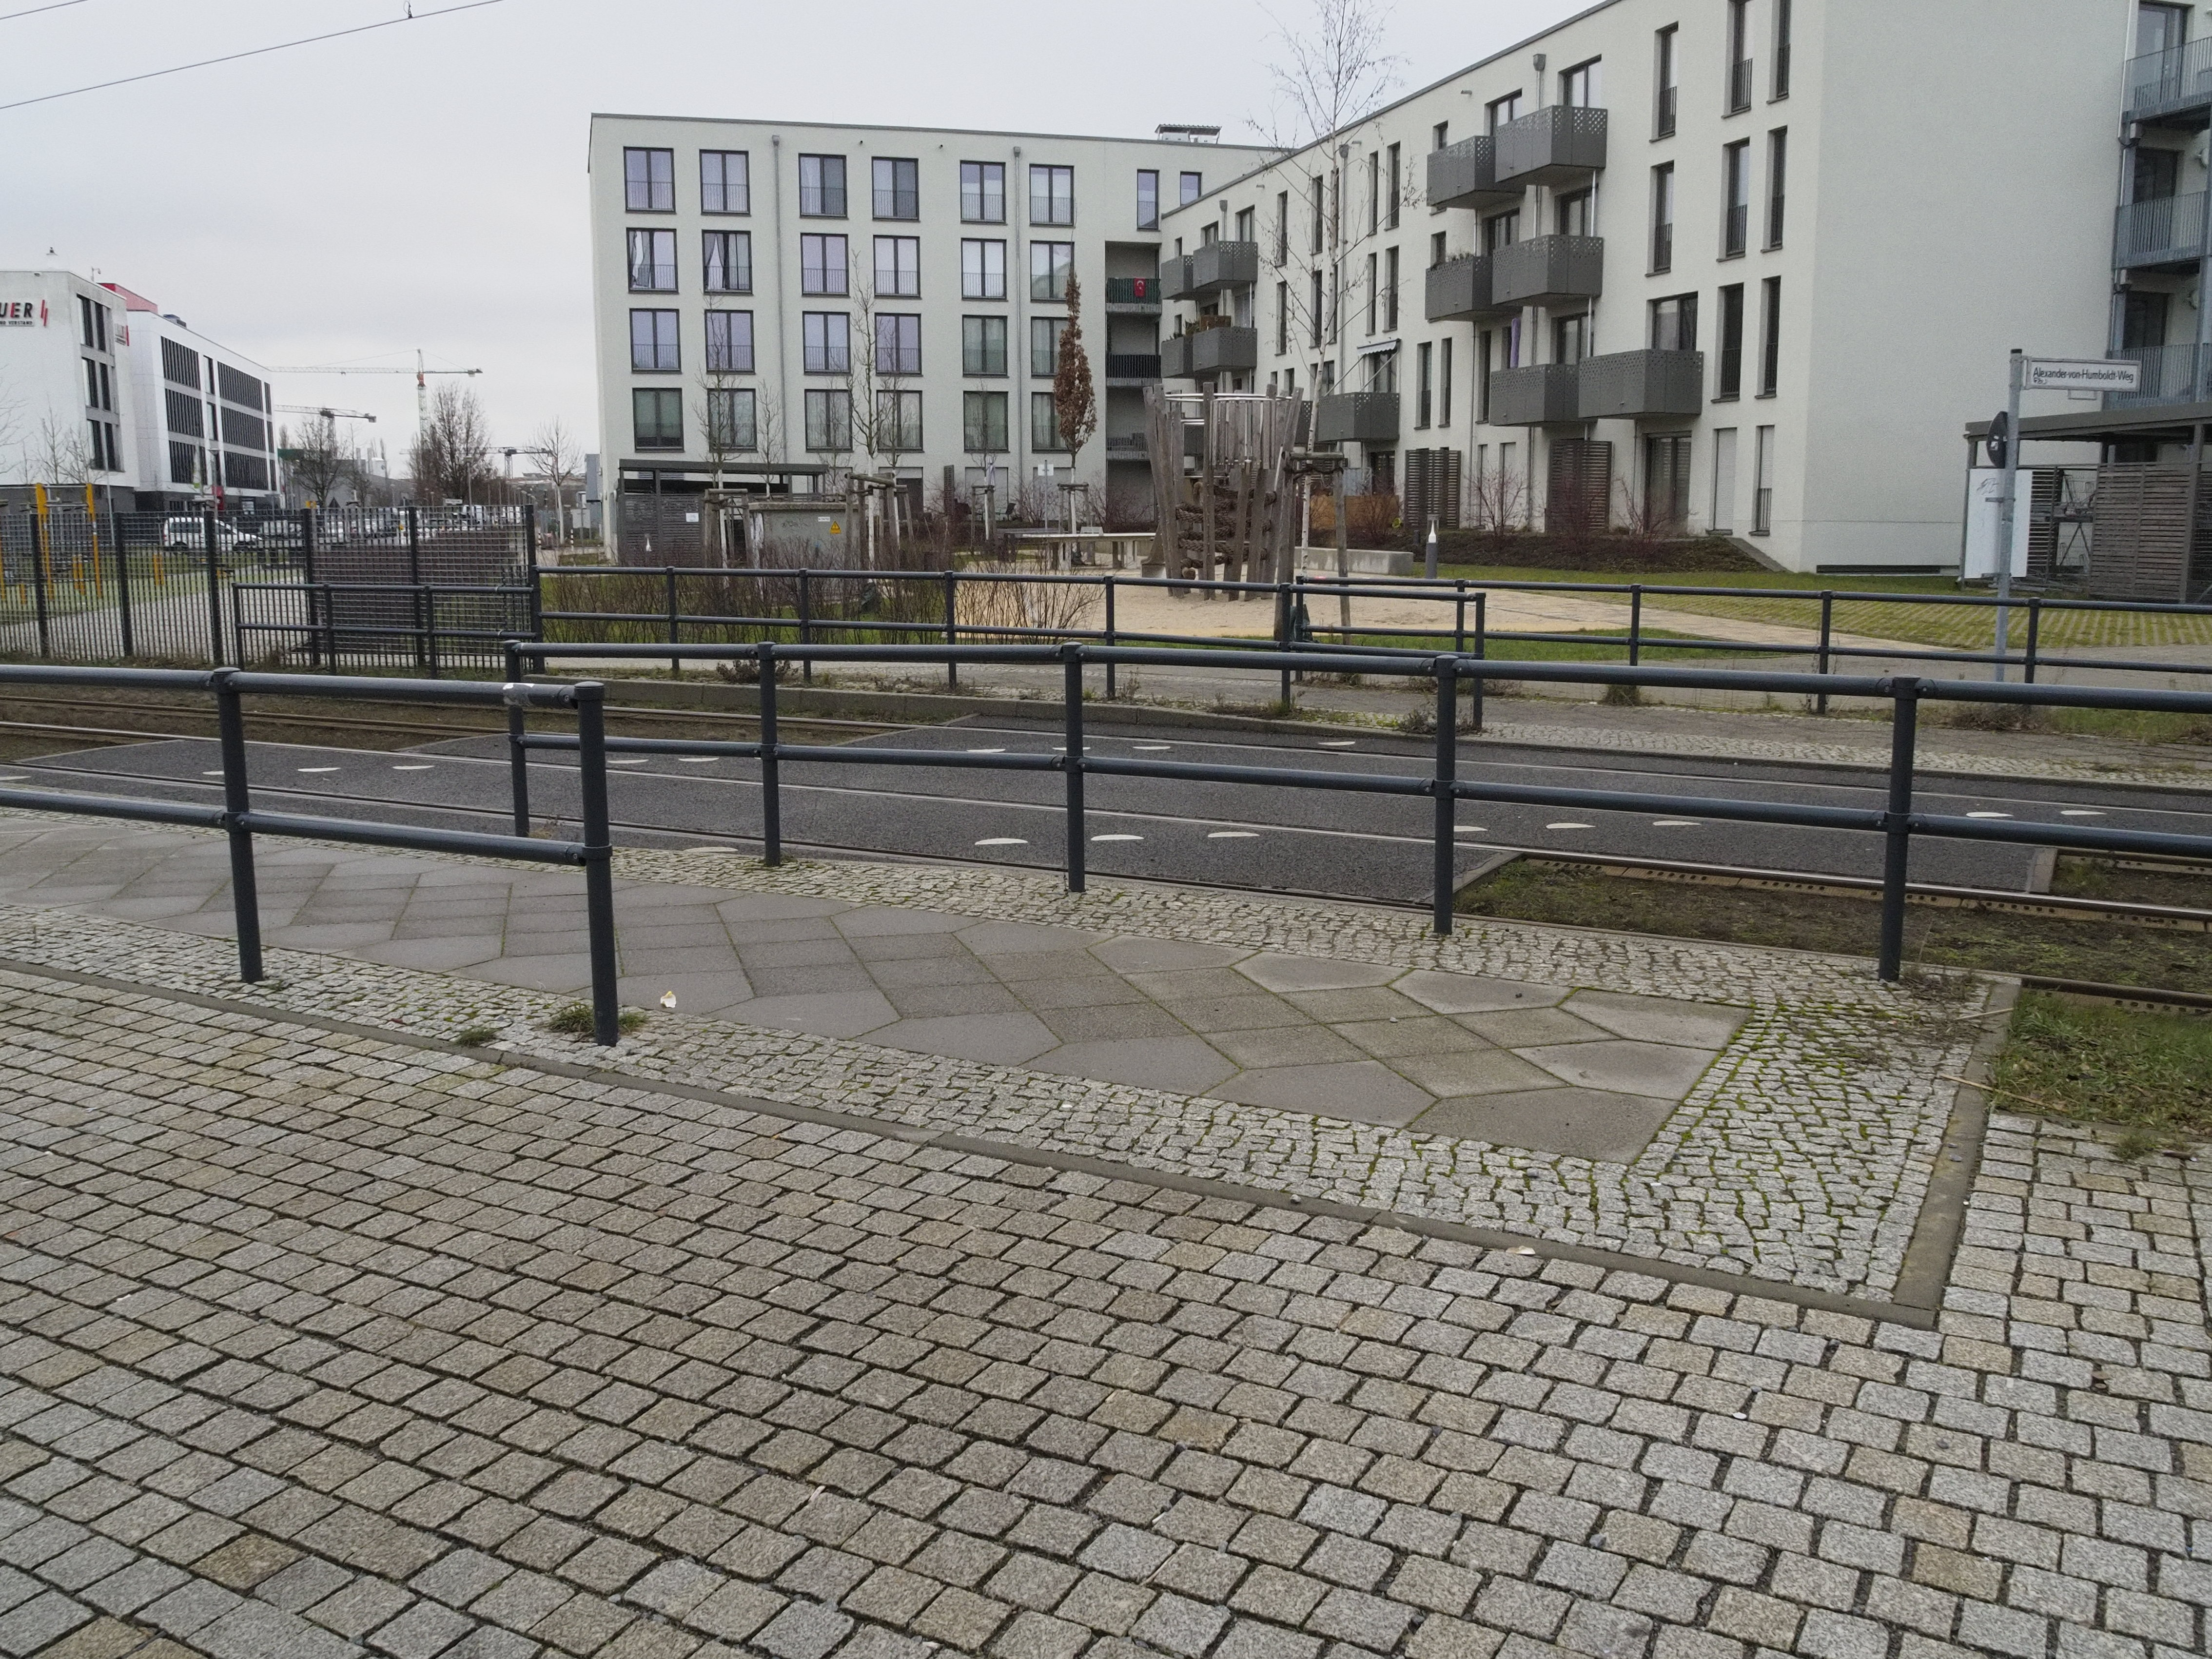
\includegraphics[width=.9333\linewidth]{images/tram_crossing.jpg}
        \caption{Tram crossing}
        \label{fig:tram_crossing}
    \end{minipage}
\end{figure}

\bigbreak\noindent
We also chose each route to contain at least one section that particularly stands out from the rest of the route.
For the “North” route this was an elevated wooden path (\autoref{fig:wood_planks}), as well as an awkward tram crossing (\autoref{fig:tram_crossing}).
The “East” route contained the objectively worst terrain of our study, a very rugged field participants had to traverse (\autoref{fig:field_east}).
The “South” route also featured an “off-road” section, traversing a lawn next to a building, this one was noticeably more flat though (\autoref{fig:field_south}).
The “East” and “South” routes also both featured different sections blocked by the same construction site (\autoref{fig:construction_site}), where participants had to result to driving on pedestrian ways.

\begin{figure}[!htb]
    \centering
    \begin{minipage}{.3333\textwidth}
        \centering
        \includegraphics[width=.9\linewidth]{images/field_east_route.jpg}
        \caption{Rugged field}
        \label{fig:field_east}
    \end{minipage}%
    \begin{minipage}{.3333\textwidth}
        \centering
        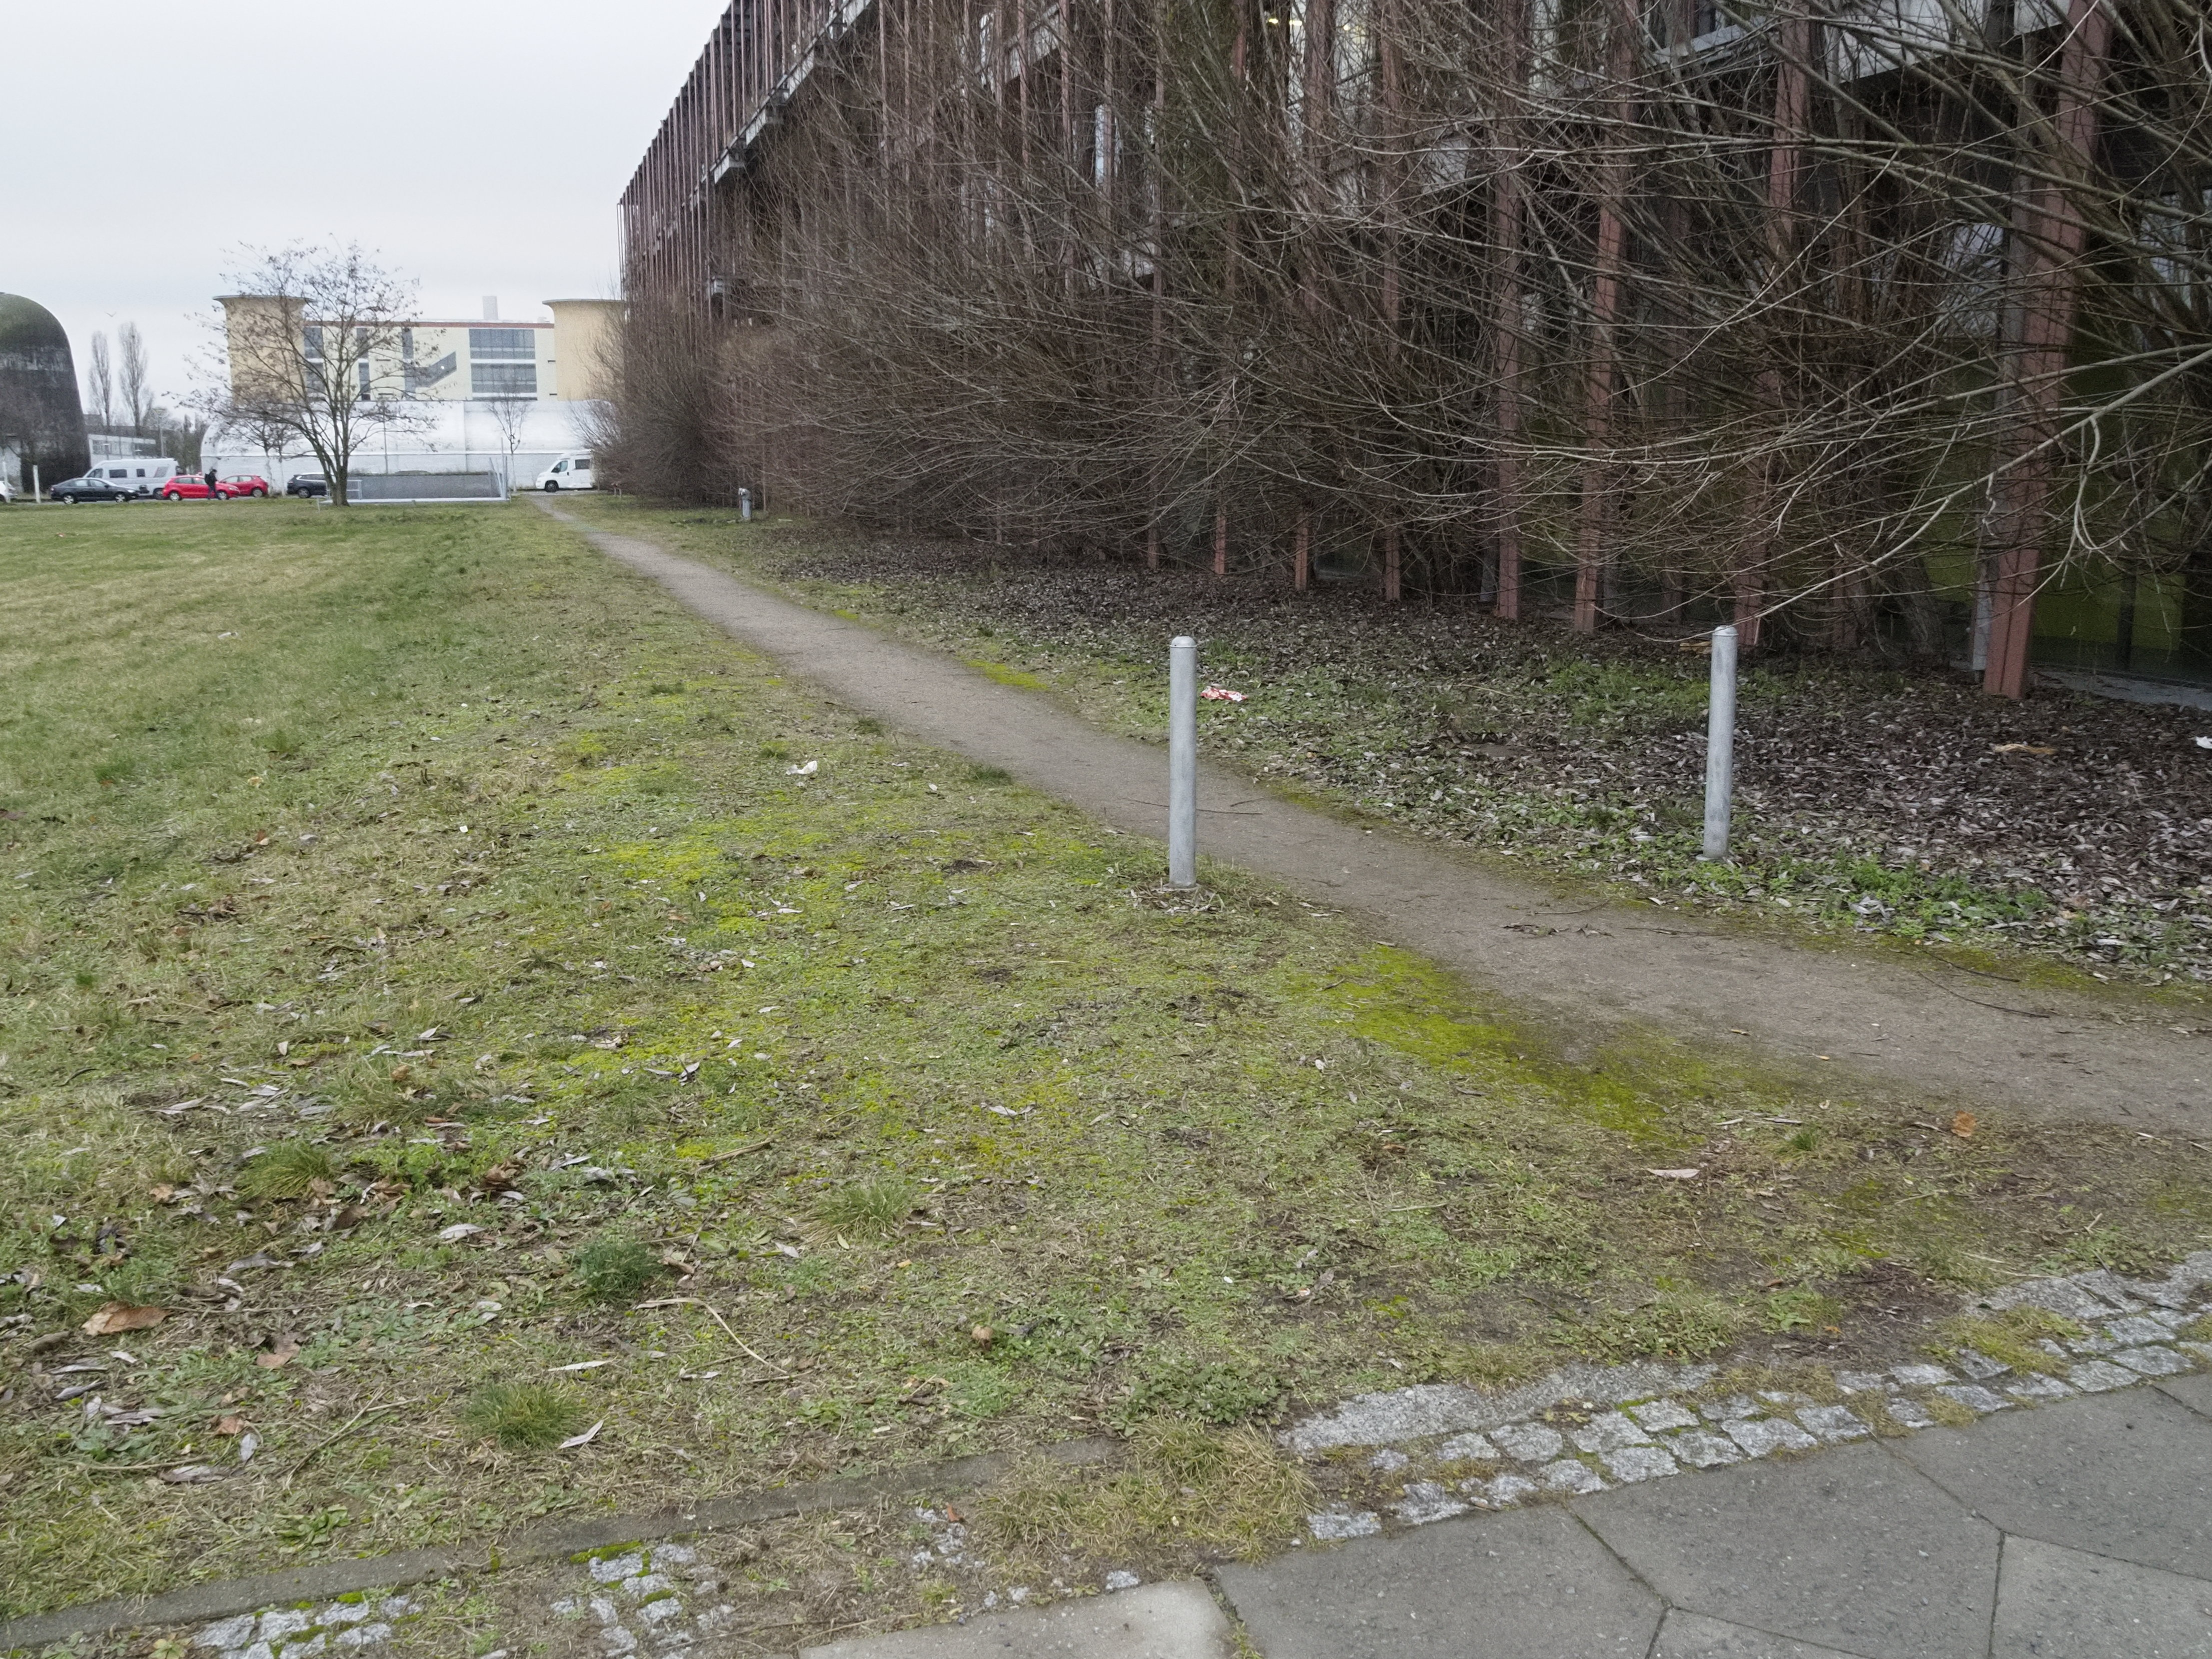
\includegraphics[width=.9\linewidth]{images/field_south_route.jpg}
        \caption{Flat lawn}
        \label{fig:field_south}
    \end{minipage}%
    \begin{minipage}{.3333\textwidth}
        \centering
        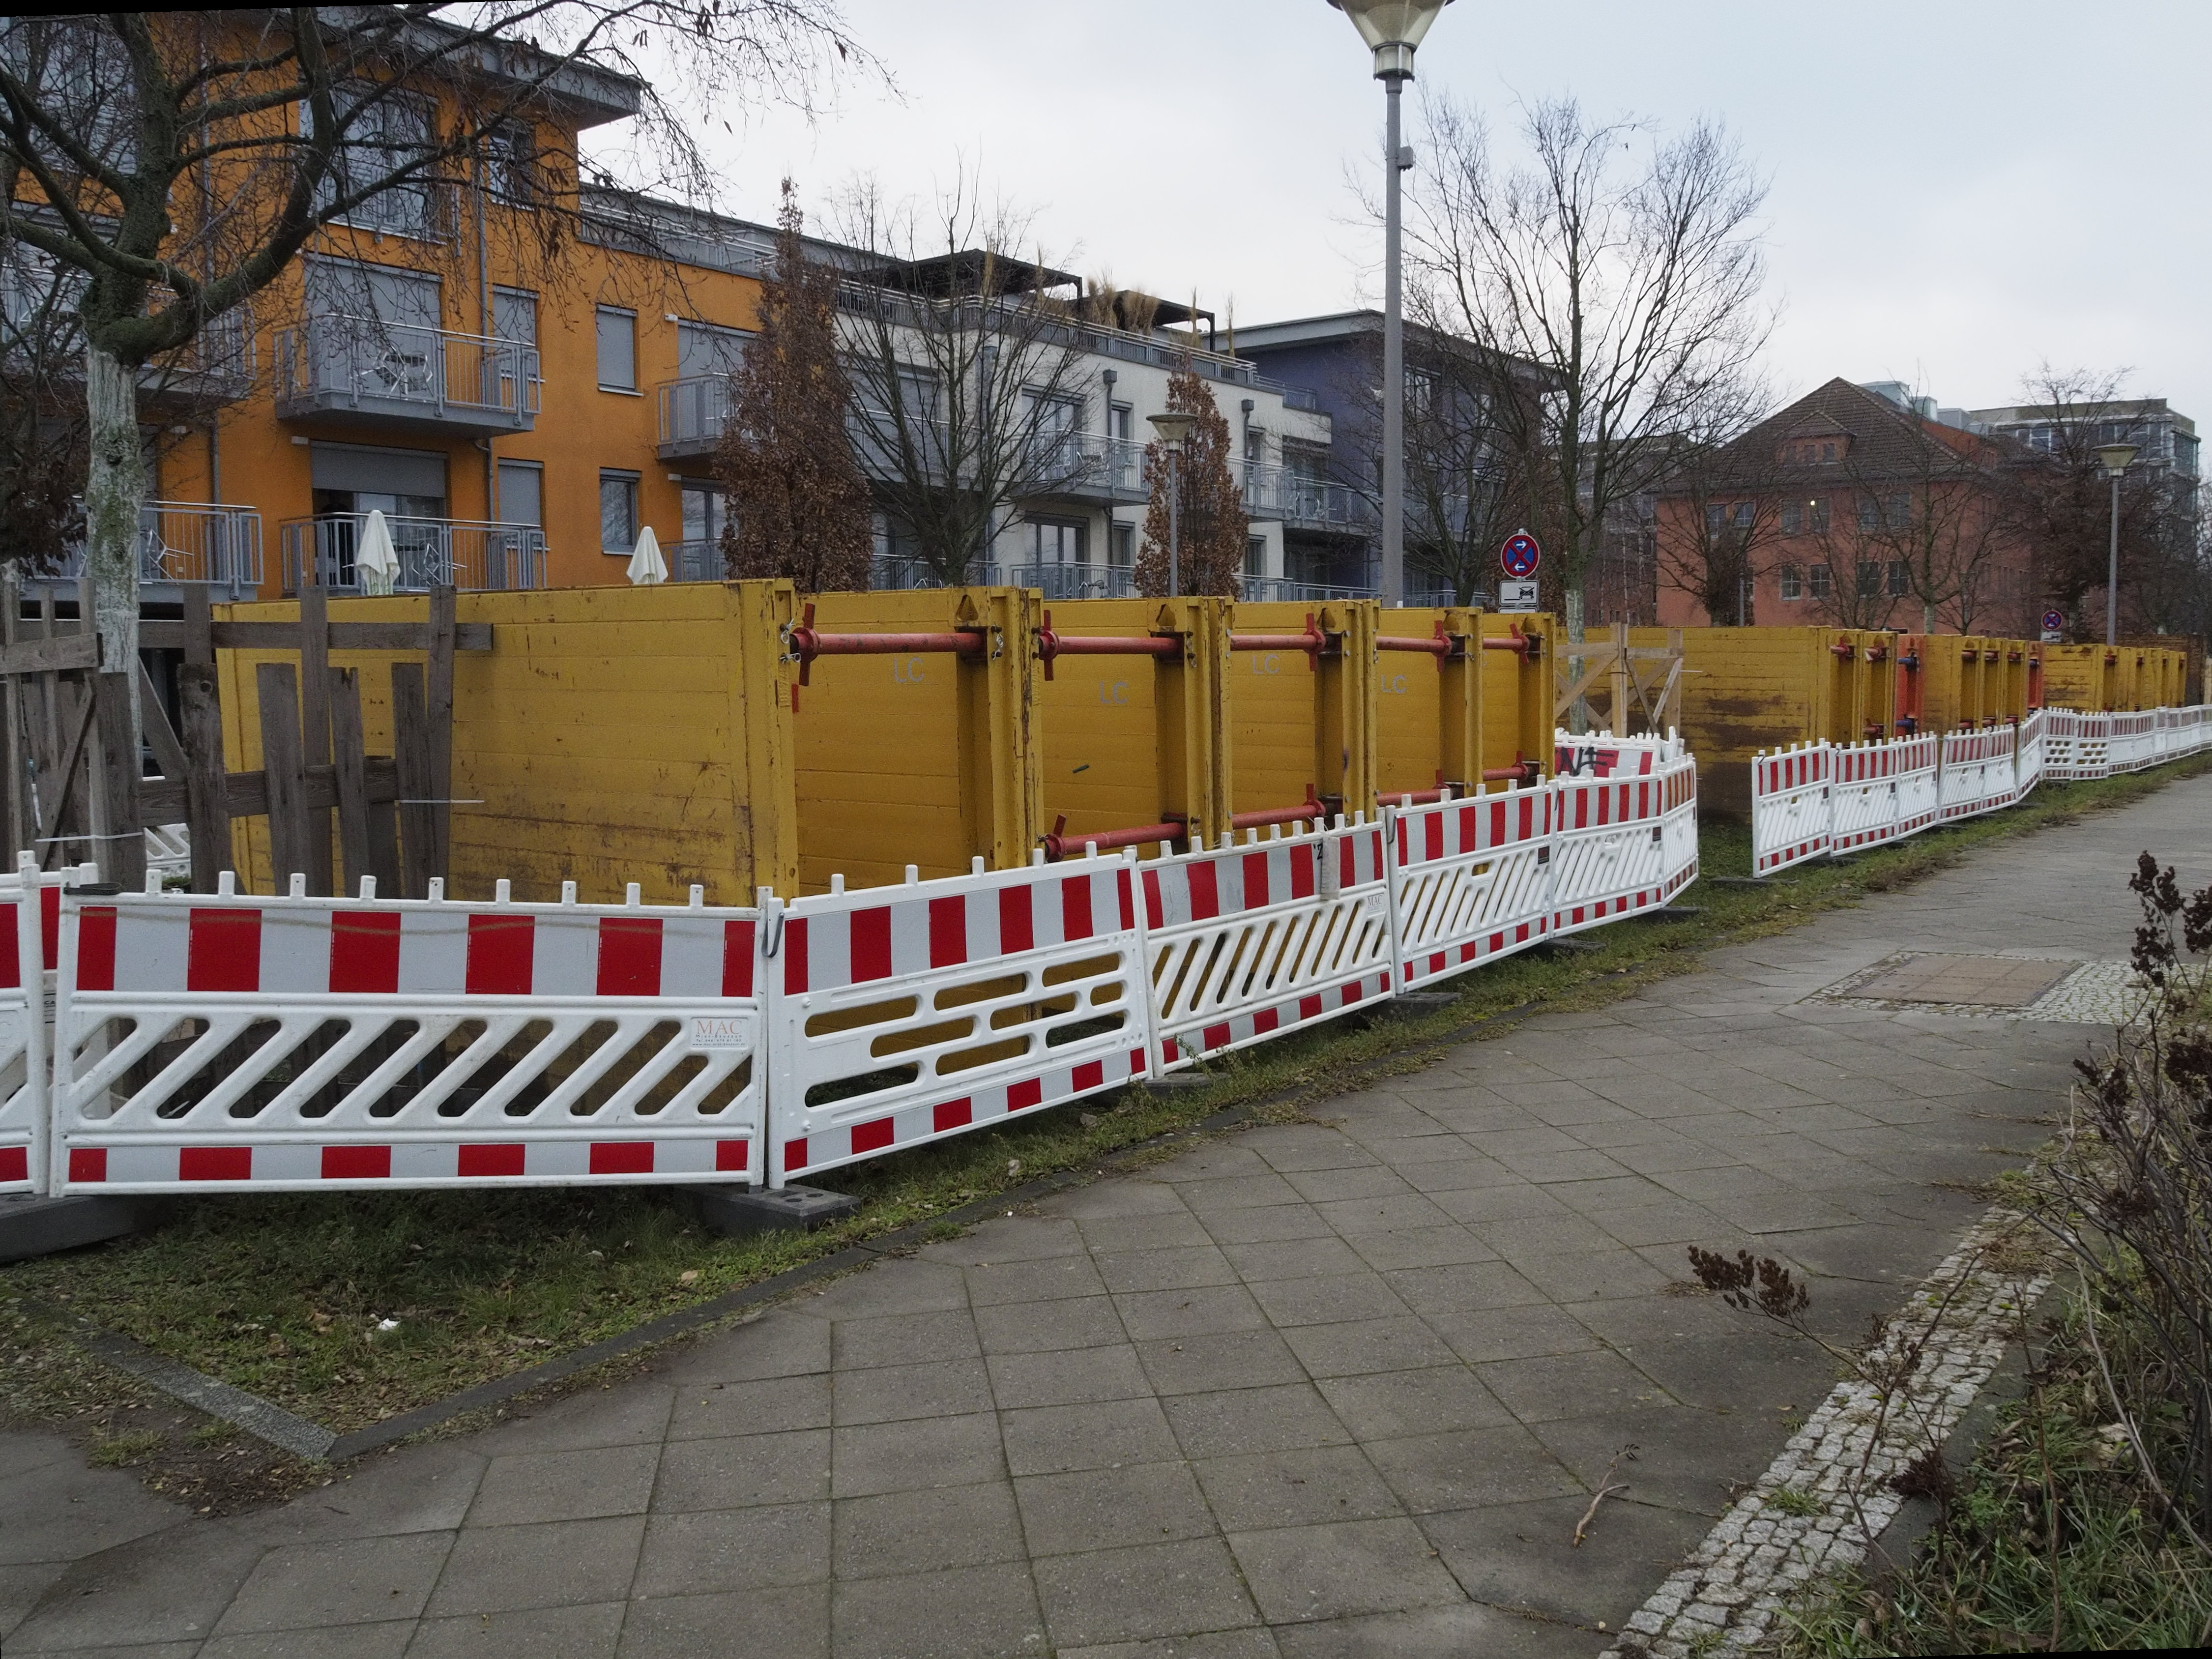
\includegraphics[width=.9\linewidth]{images/construction_site.jpg}
        \caption{Construction site}
        \label{fig:construction_site}
    \end{minipage}
\end{figure}

\subsection{Data Collection}\label{subsec:data_collection}

All data was collected using the \likertshift app acting as a frontend for our prototype, as described in \autoref{subsec:frontend_design} and the \audiorecording and \mapping methods were added to it.
\audiorecording is implemented by using the smartphones internal microphone to record an audio track while cycling.
The recorded audio will then be added to the recording data as a lossless \texttt{FLAC} file.
For the \mapping method, we only recorded location and time information in the app.
The actual ratings were performed retrospectively on a piece of paper.
After resetting the app at the end of each study participation, we simply wrote down the participants ID on said piece of paper, to be able to match it with the recorded data later on.
This is described in more detail in \autoref{subsec:preprocessing}.

\subsubsection{Questionnaires}

In addition to this quantitative data, we also used two questionnaires, the \citetext{nasa_tlx}{NASA TLX} and the \citetext{ueq+}{UEQ+} (a modular extension of the commonly used \citetext{ueq}{UEQ}) to obtain qualitative data, regarding differences between the recording methods used.
Participants were asked to fill in these questionnaires right after they finished rating a route with each method.
We made sure participants understood that both questionnaires only concerned the respective method used to rate their subjective experience during cycling, but not the act of cycling itself.
For the \citetextnoref{ueq+}{UEQ+}, we selected the \textit{Attractiveness}, \textit{Efficiency}, \textit{Intuitive Use}, \textit{Hardware Security} and \textit{Social Acceptance} scales and slightly adjusted some questions wordings, as the \citetextnoref{ueq+}{UEQ+} is usually used to evaluate the user experience of products, not methods.

\subsubsection{Interview}

We also conducted a short $\sim\SI{10}{min}$ interview with every participant, asking them about their frequency of and reasoning for cycling, a ranking of the three methods used to record their subjective experience, as well as problems that could occur and possible improvements for each of the methods.
Additionally, we asked what kind of bicycles participants used privately and whether our devices would be able to be mounted to them in its current form, to assess the compatibility of our method with different types of bicycles.

\subsection{Procedure}

We started by giving an introduction to the study as well as the methods used and explained the general order of operations and approximate duration.
We also provided participants with an informed consent sheet, outlining the procedure, associated risks, our data protection guidelines and information about compensation, which they had to sign.
They then got introduced to out \likertshift app and had to fill in the initial demographics form.
Next, participants were shown the bicycle used for performing the study (\autoref{fig:study_bike}) and then asked to adjust the saddle height to their liking and to drive along a short test route, to get used to it.
Then, we randomly selected a row from our balancing sheet (containing three method/route combinations, with each method and route only appearing once).
For each of these combinations, we first explained the method used to participants and asked them if they would like to perform another short test drive to simulate using said method.
Once done, participants drove the respective route and after submitting their ratings, also filled in our prepared questionnaires in the \likertshift app.
During the ride, a smartphone was mounted to the bicycle, in between the handlebars (\autoref{fig:smartphone_holder}), running the \likertshift app which displayed the route participants had to follow and recorded the required data.
After all three combinations were completed, we finished by carrying out our interview.
Finally, each participant received a compensation of \euro10.00 for their efforts.

% linewidth_factor = 1 - (1 / (30 * textwidth_factor))
% textwidth_factor ~ 4/7 (adjusted by hand)
\begin{figure}[!htb]
    \centering
    \begin{minipage}{.5675\textwidth}
        \centering
        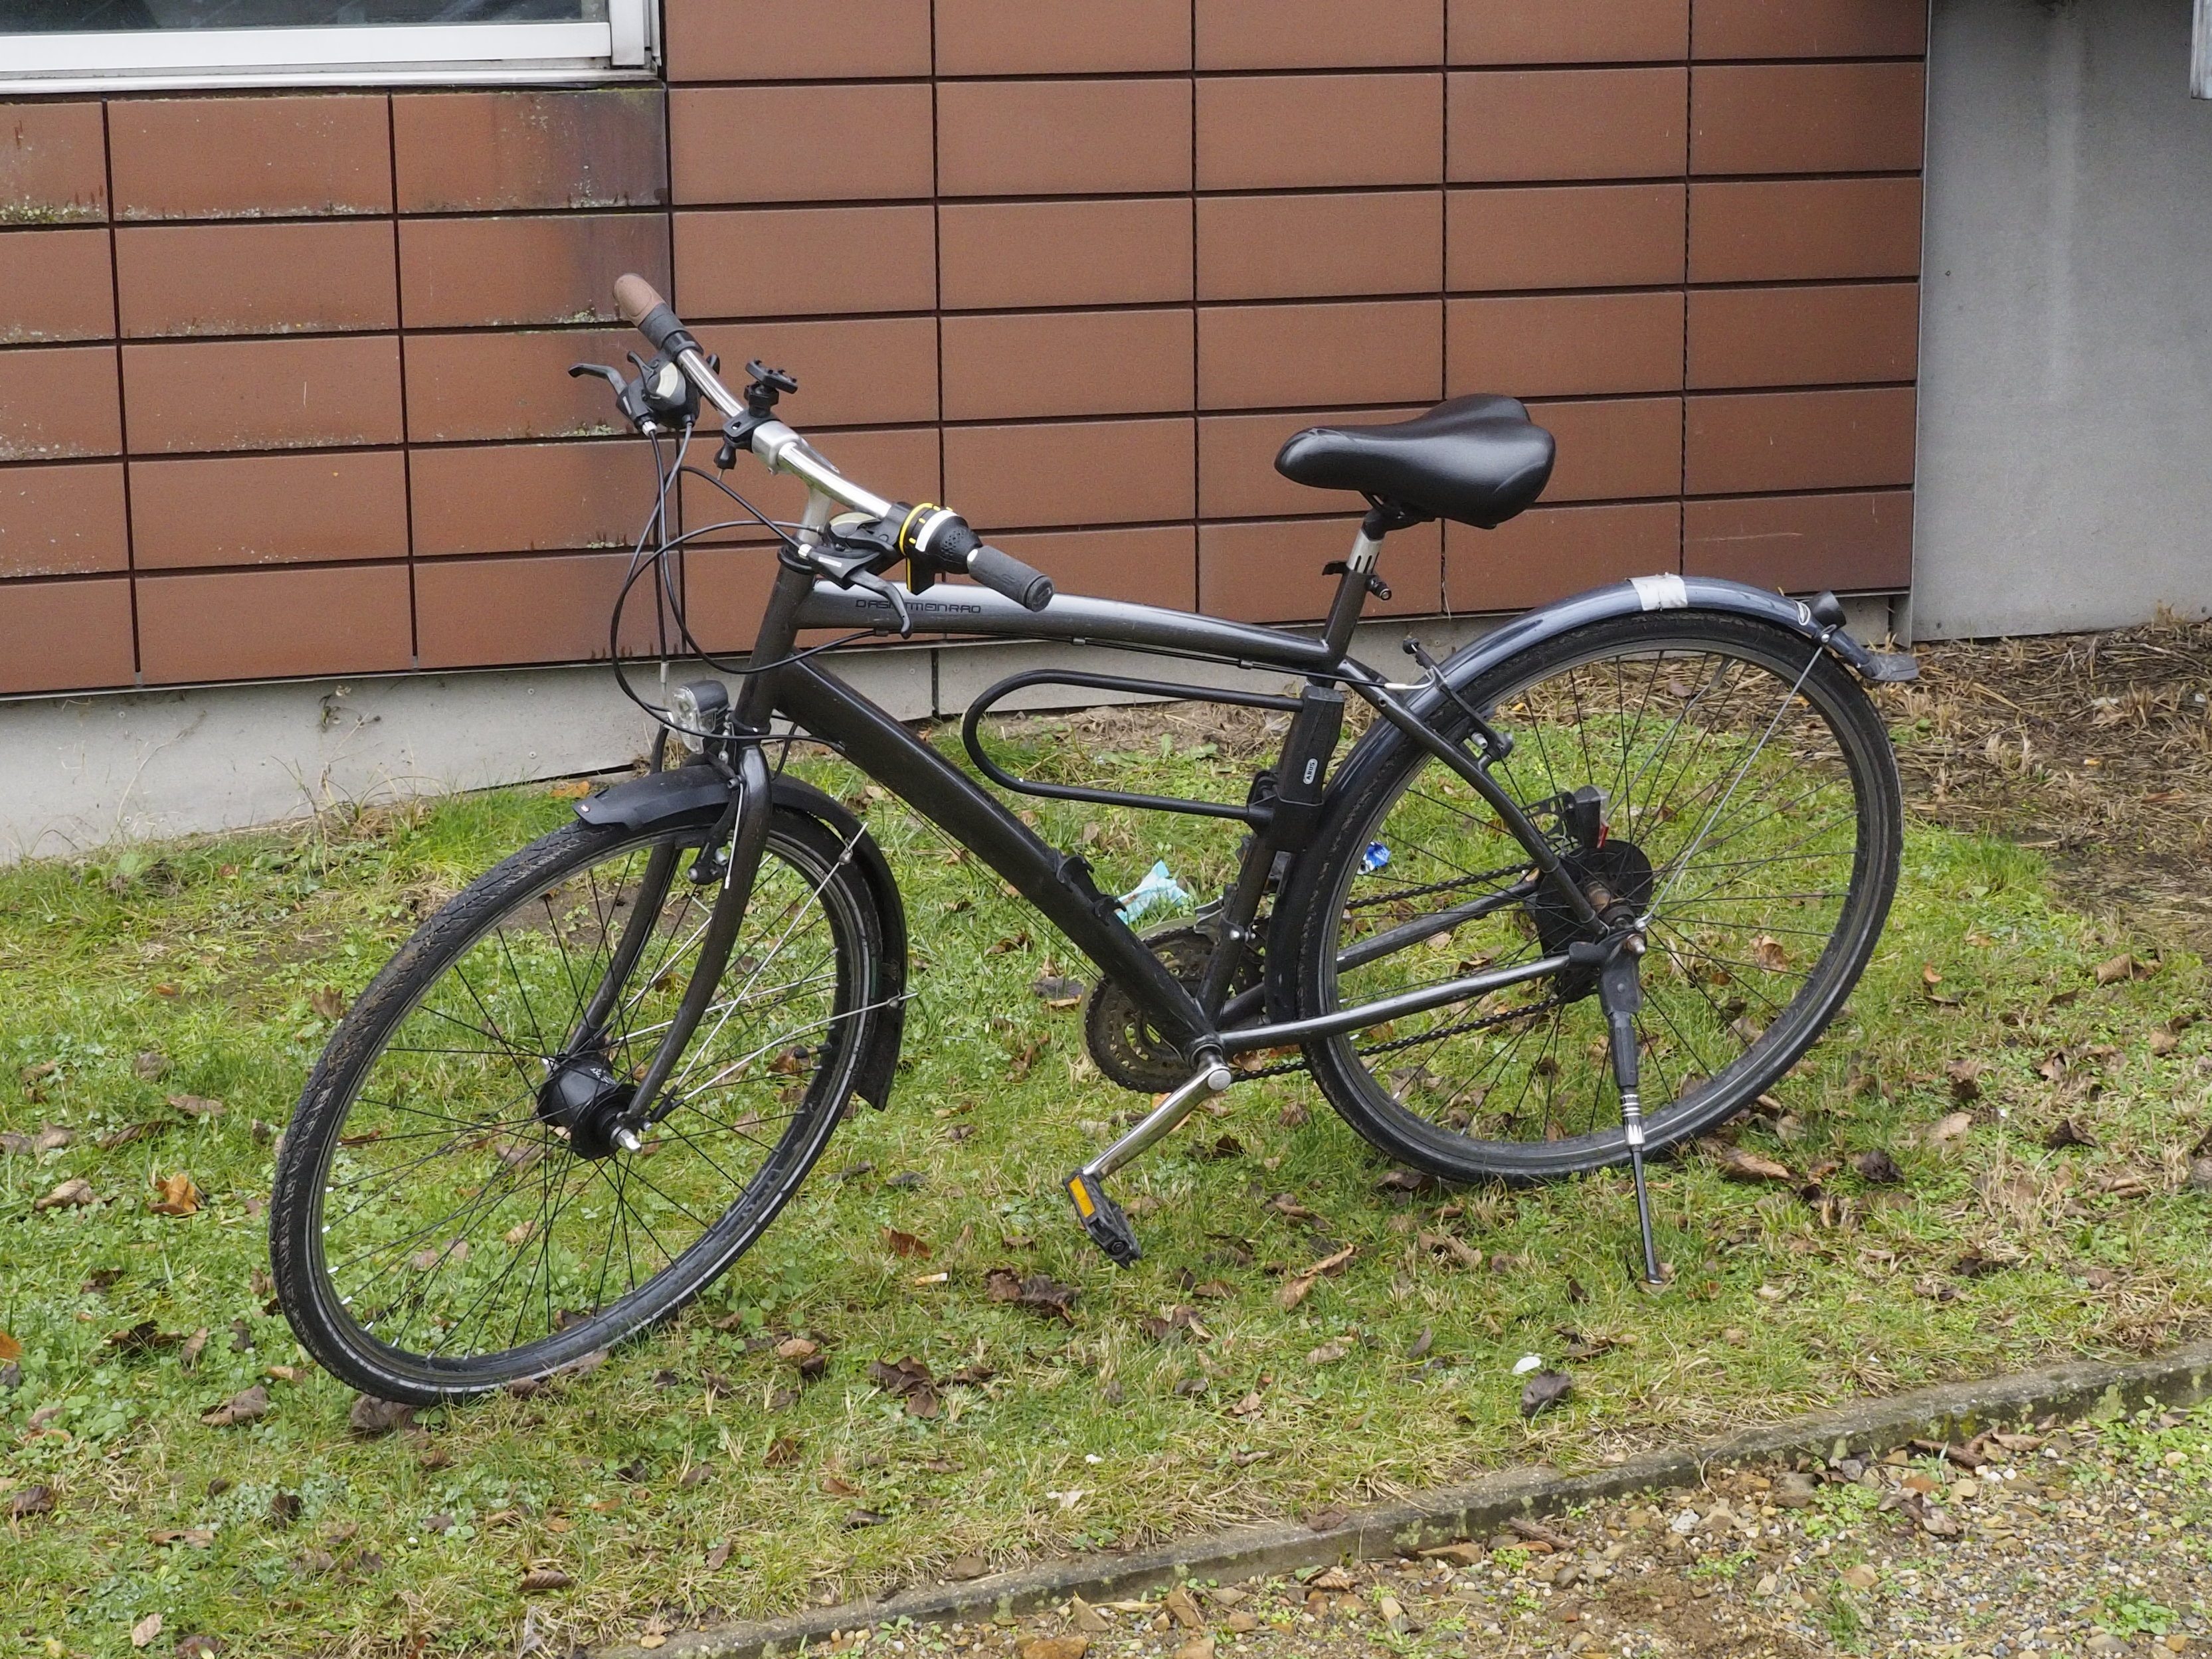
\includegraphics[width=.9413\linewidth]{images/study_bike.jpg}
        \caption{The bicycle used in the field-study}
        \label{fig:study_bike}
    \end{minipage}%
    \begin{minipage}{.4325\textwidth}
        \centering
        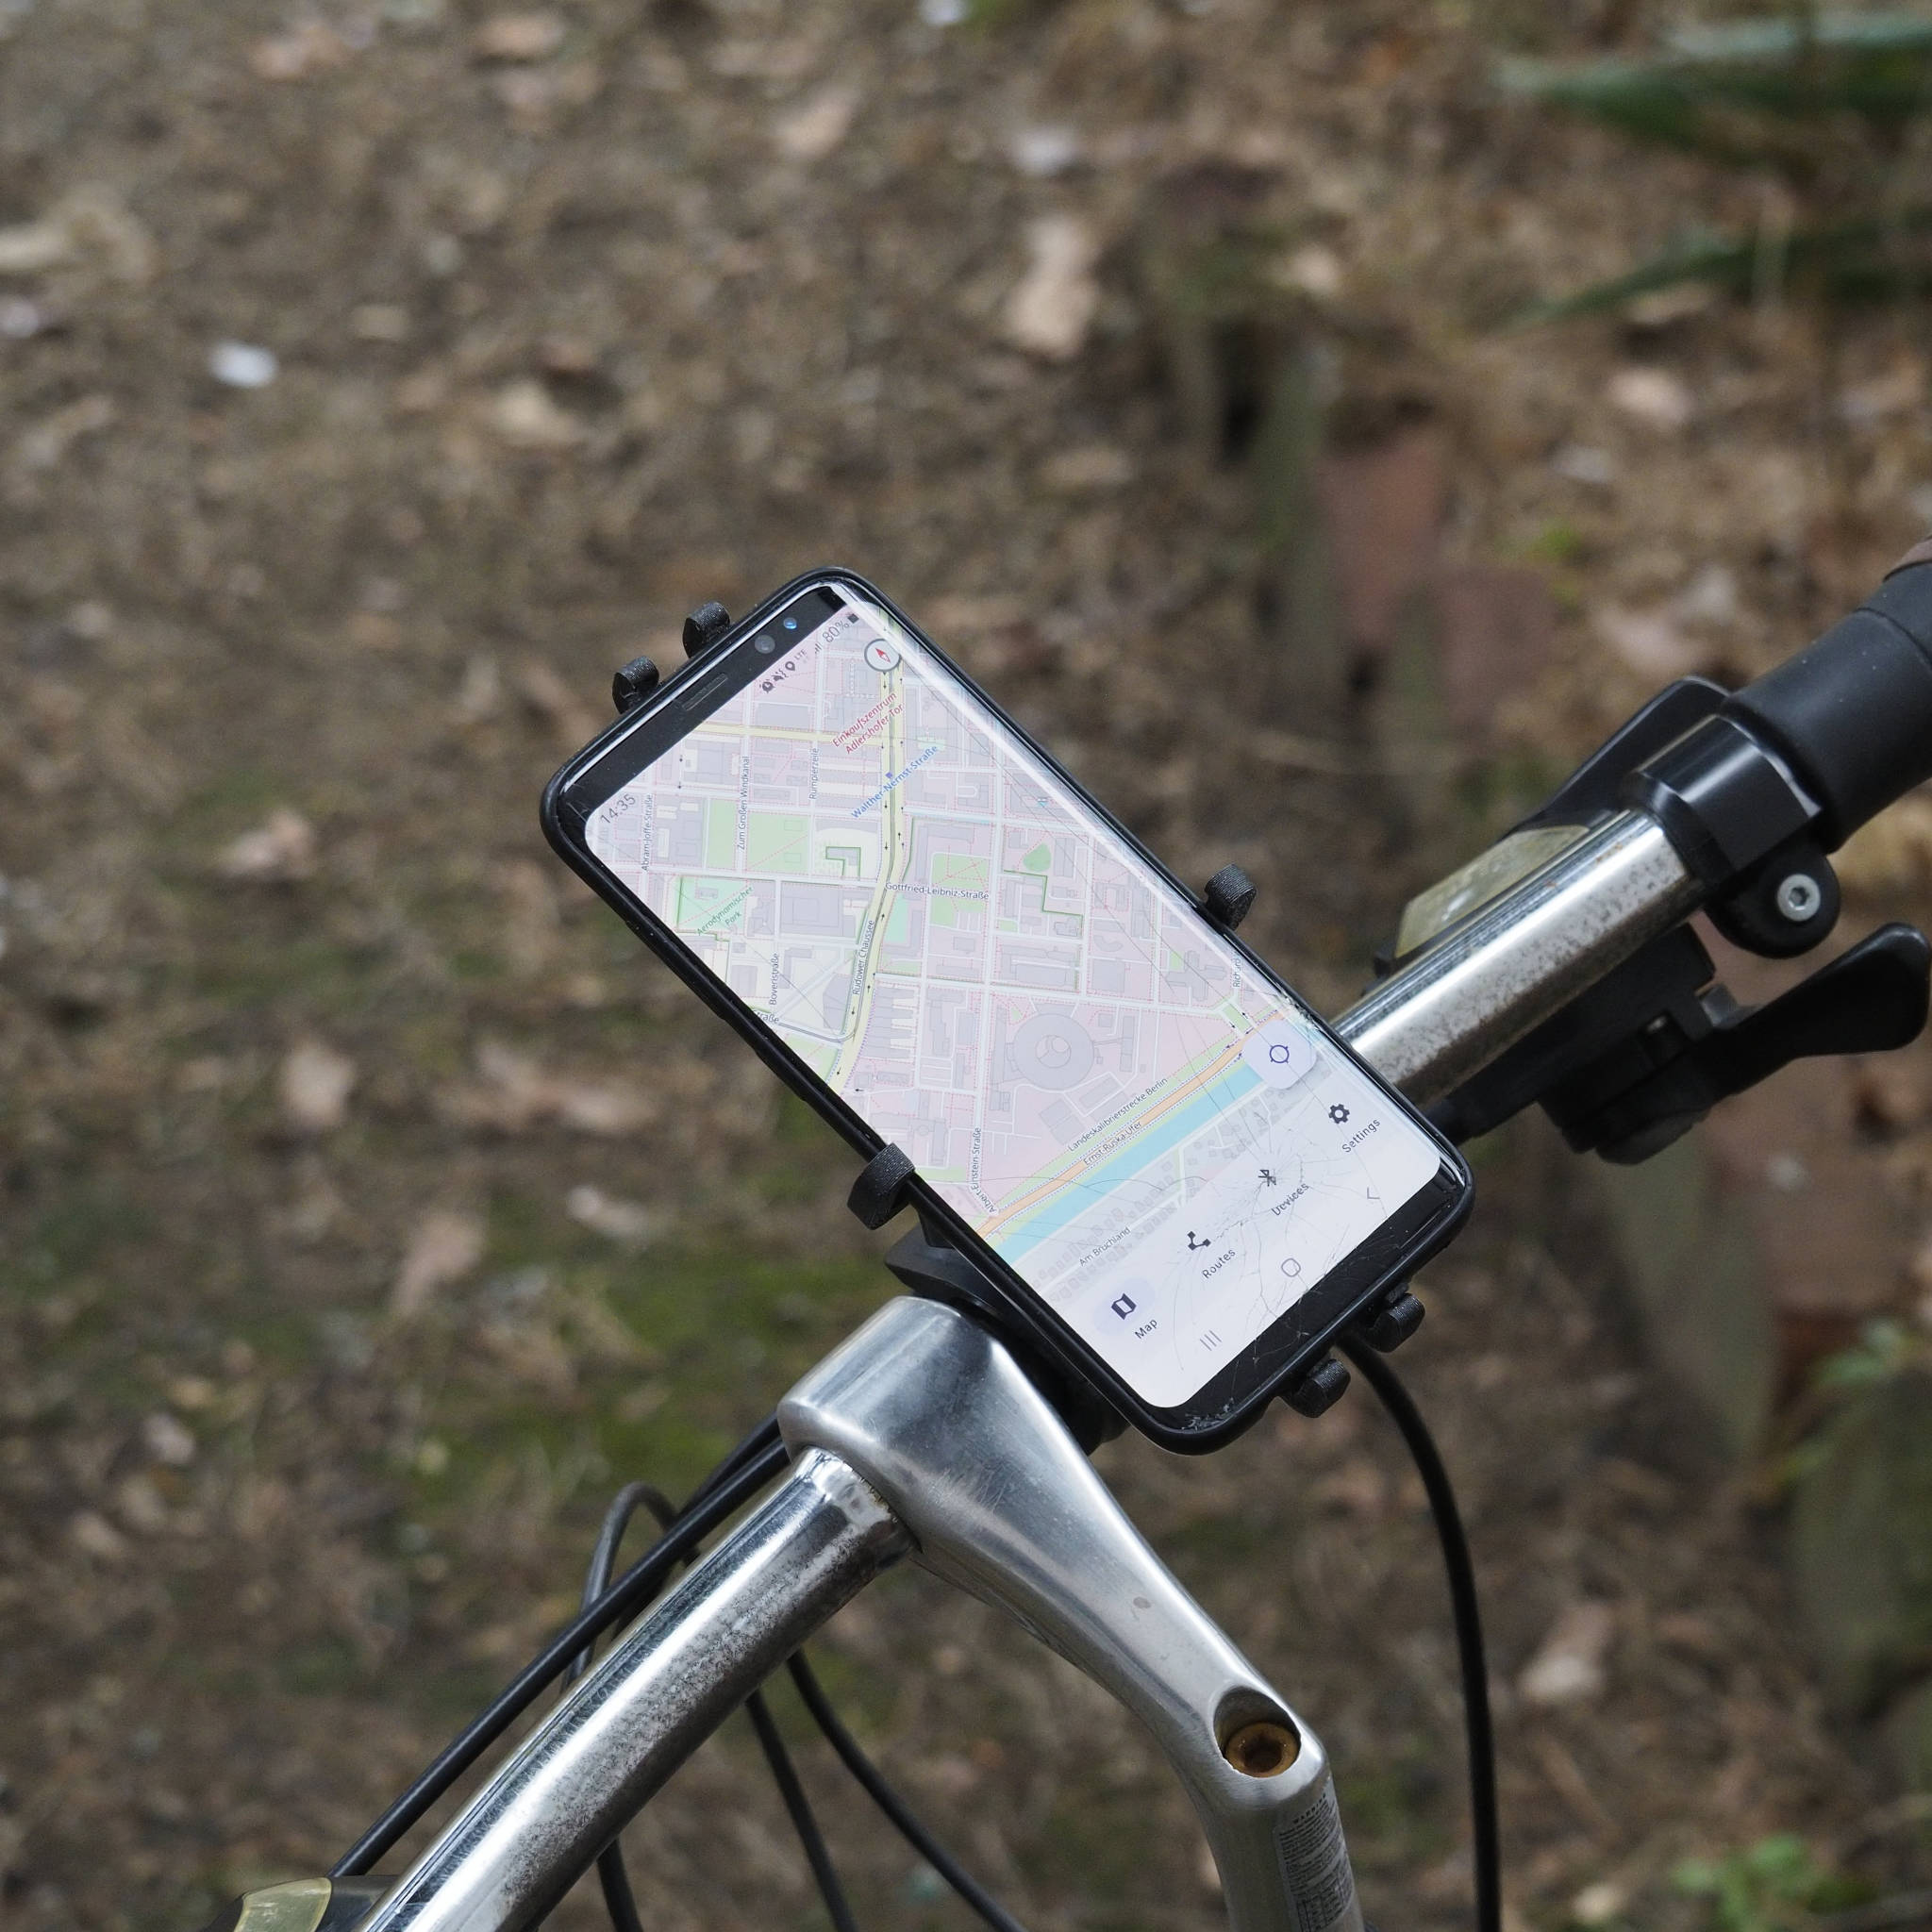
\includegraphics[width=.9229\linewidth]{images/smartphone_holder.jpg}
        \caption{Smartphone holder}
        \label{fig:smartphone_holder}
    \end{minipage}
\end{figure}

\subsubsection*{Safety Precautions}

To ensure each participants' safety, the researcher conducting the study followed them on their routes, retaining a save distance, with another bicycle.
Participants were further told to not look at the route on the smartphone for extended periods of time and to focus their attention on the road in front of them and to stop and get in contact with the researcher if a problem occurred, but to otherwise ignore them.
They were also told to only drive at a conservative, safe speed.

\newpage\section{Results}\label{sec:results}

\subsection{Participants}

We recruited a total of 18 participants for our study using posters we placed on the university campus in combination with snowball sampling.
Participants age ranged from 18 to 59 years and only 3 of the 18 participants identified as female, all others identified as male.
Each participant received a compensation of \euro10.00 for their efforts.
The study was conducted from November to December, but except for temperature differences and some light raining, general weather conditions were consistent between study sessions.
Each session to about 90 minutes in total.
We experienced no study cancellations and all recorded data was useable.

\subsection{Route Data}

In this section we describe the evaluation of the quantitative ratings performed by participants on the measure of “Travel satisfaction, based on the road” using the \likertshift, \audiorecording, and \mapping methods respectively, as described in \autoref{subsec:recording_methods} and \autoref{subsec:data_collection}. \autoref{fig:route_ratings} shows a visually appealing overview of all data collected using all three methods.

\begin{figure}[!htb]
    \centering
    \begin{subfigure}{.3333\textwidth}
        \centering
        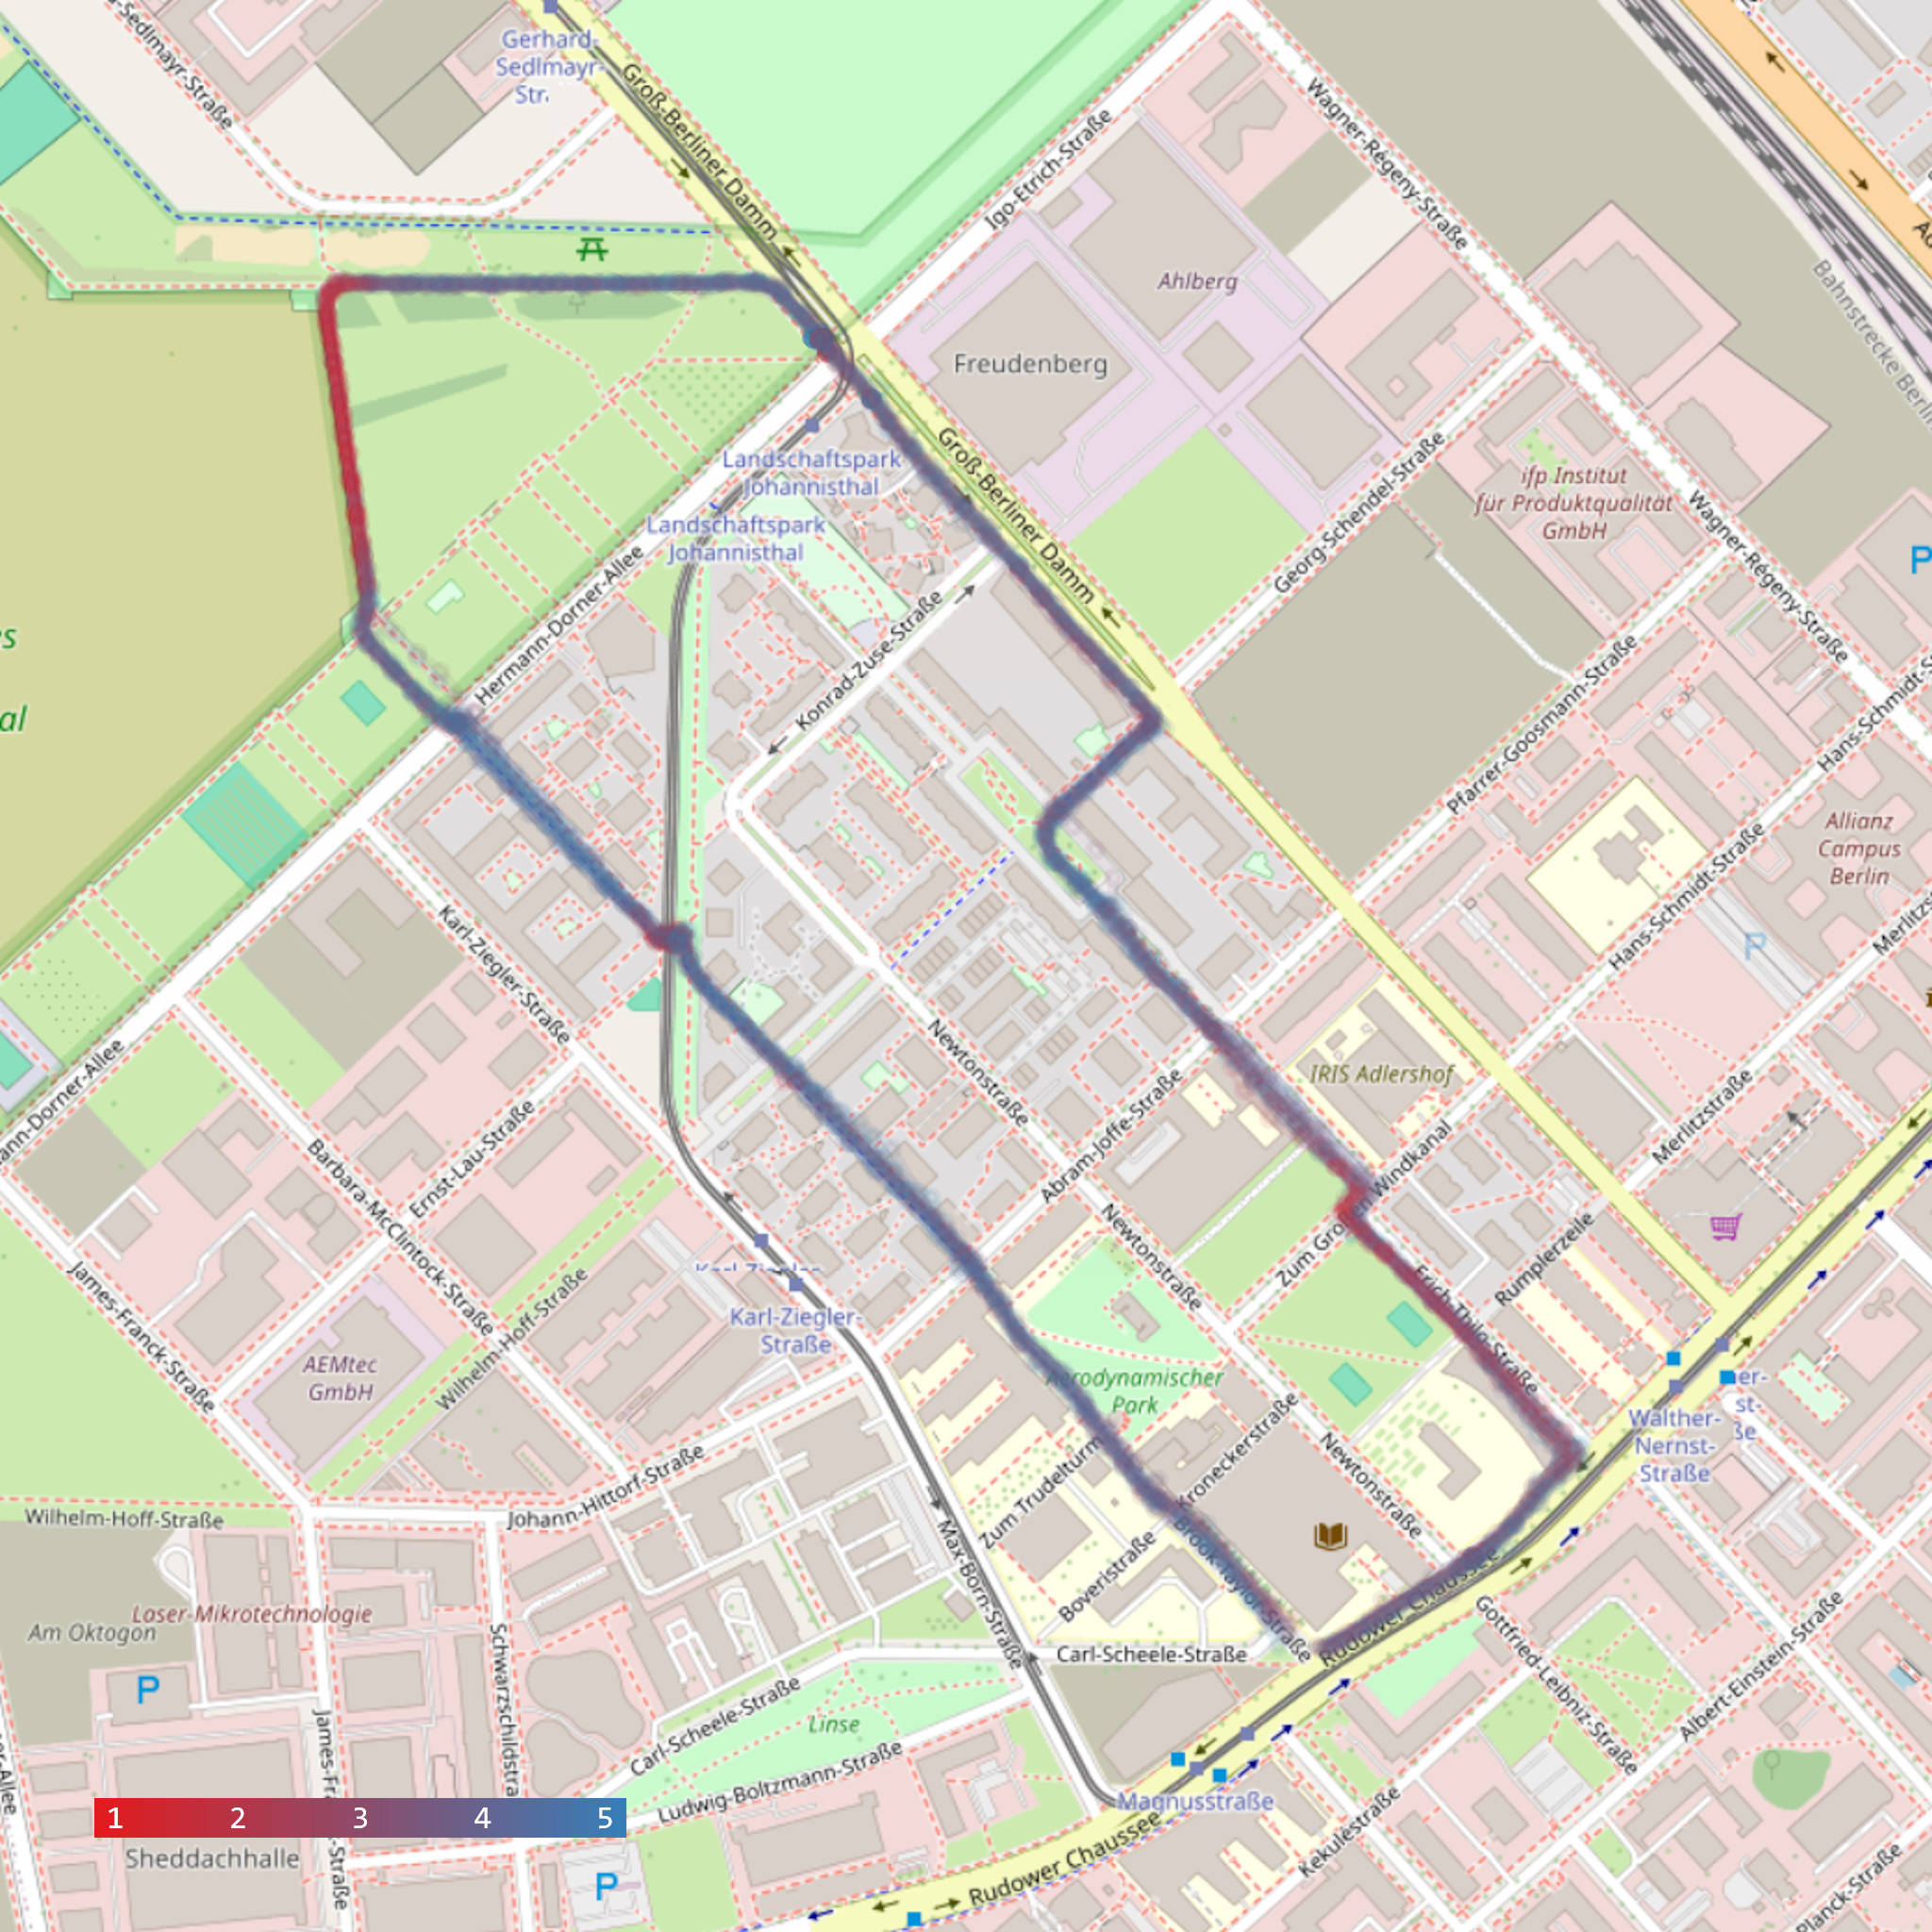
\includegraphics[width=.9\linewidth]{images/ratings_north_route.jpg}
        \caption{North route}
        \label{fig:ratings_north_route}
    \end{subfigure}%
    \begin{subfigure}{.3333\textwidth}
        \centering
        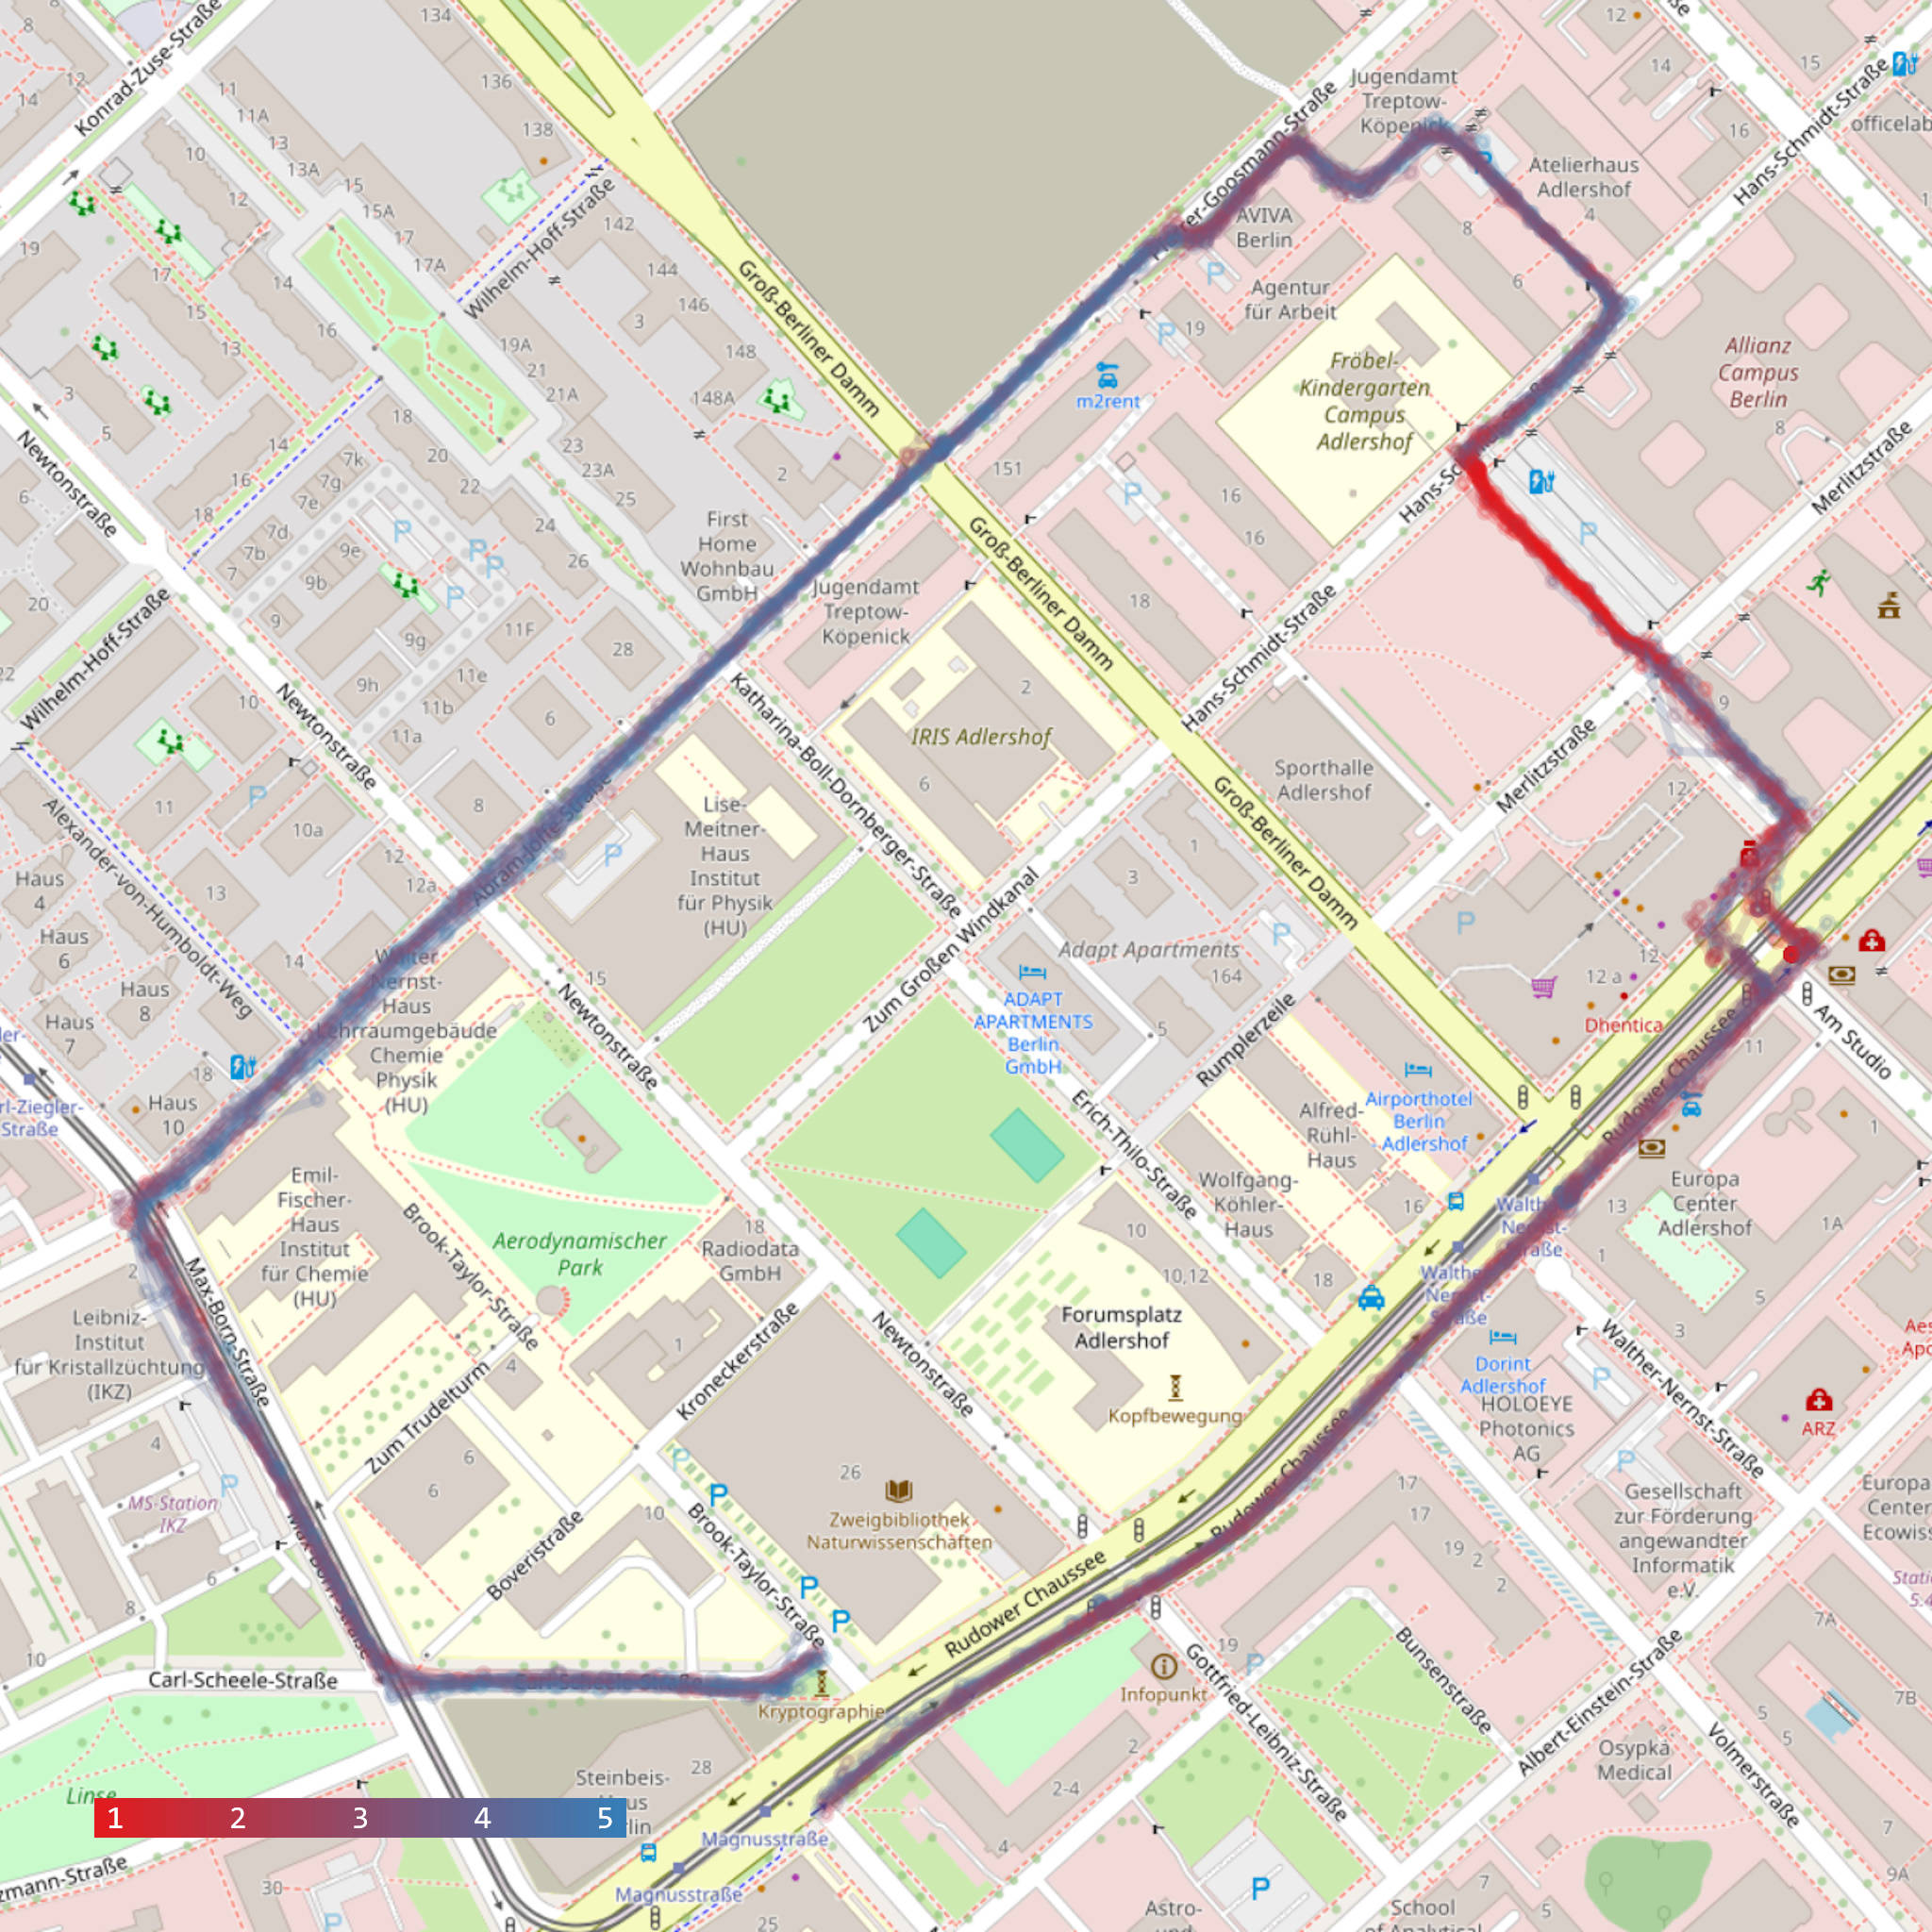
\includegraphics[width=.9\linewidth]{images/ratings_east_route.jpg}
        \caption{East route}
        \label{fig:ratings_east_route}
    \end{subfigure}%
    \begin{subfigure}{.3333\textwidth}
        \centering
        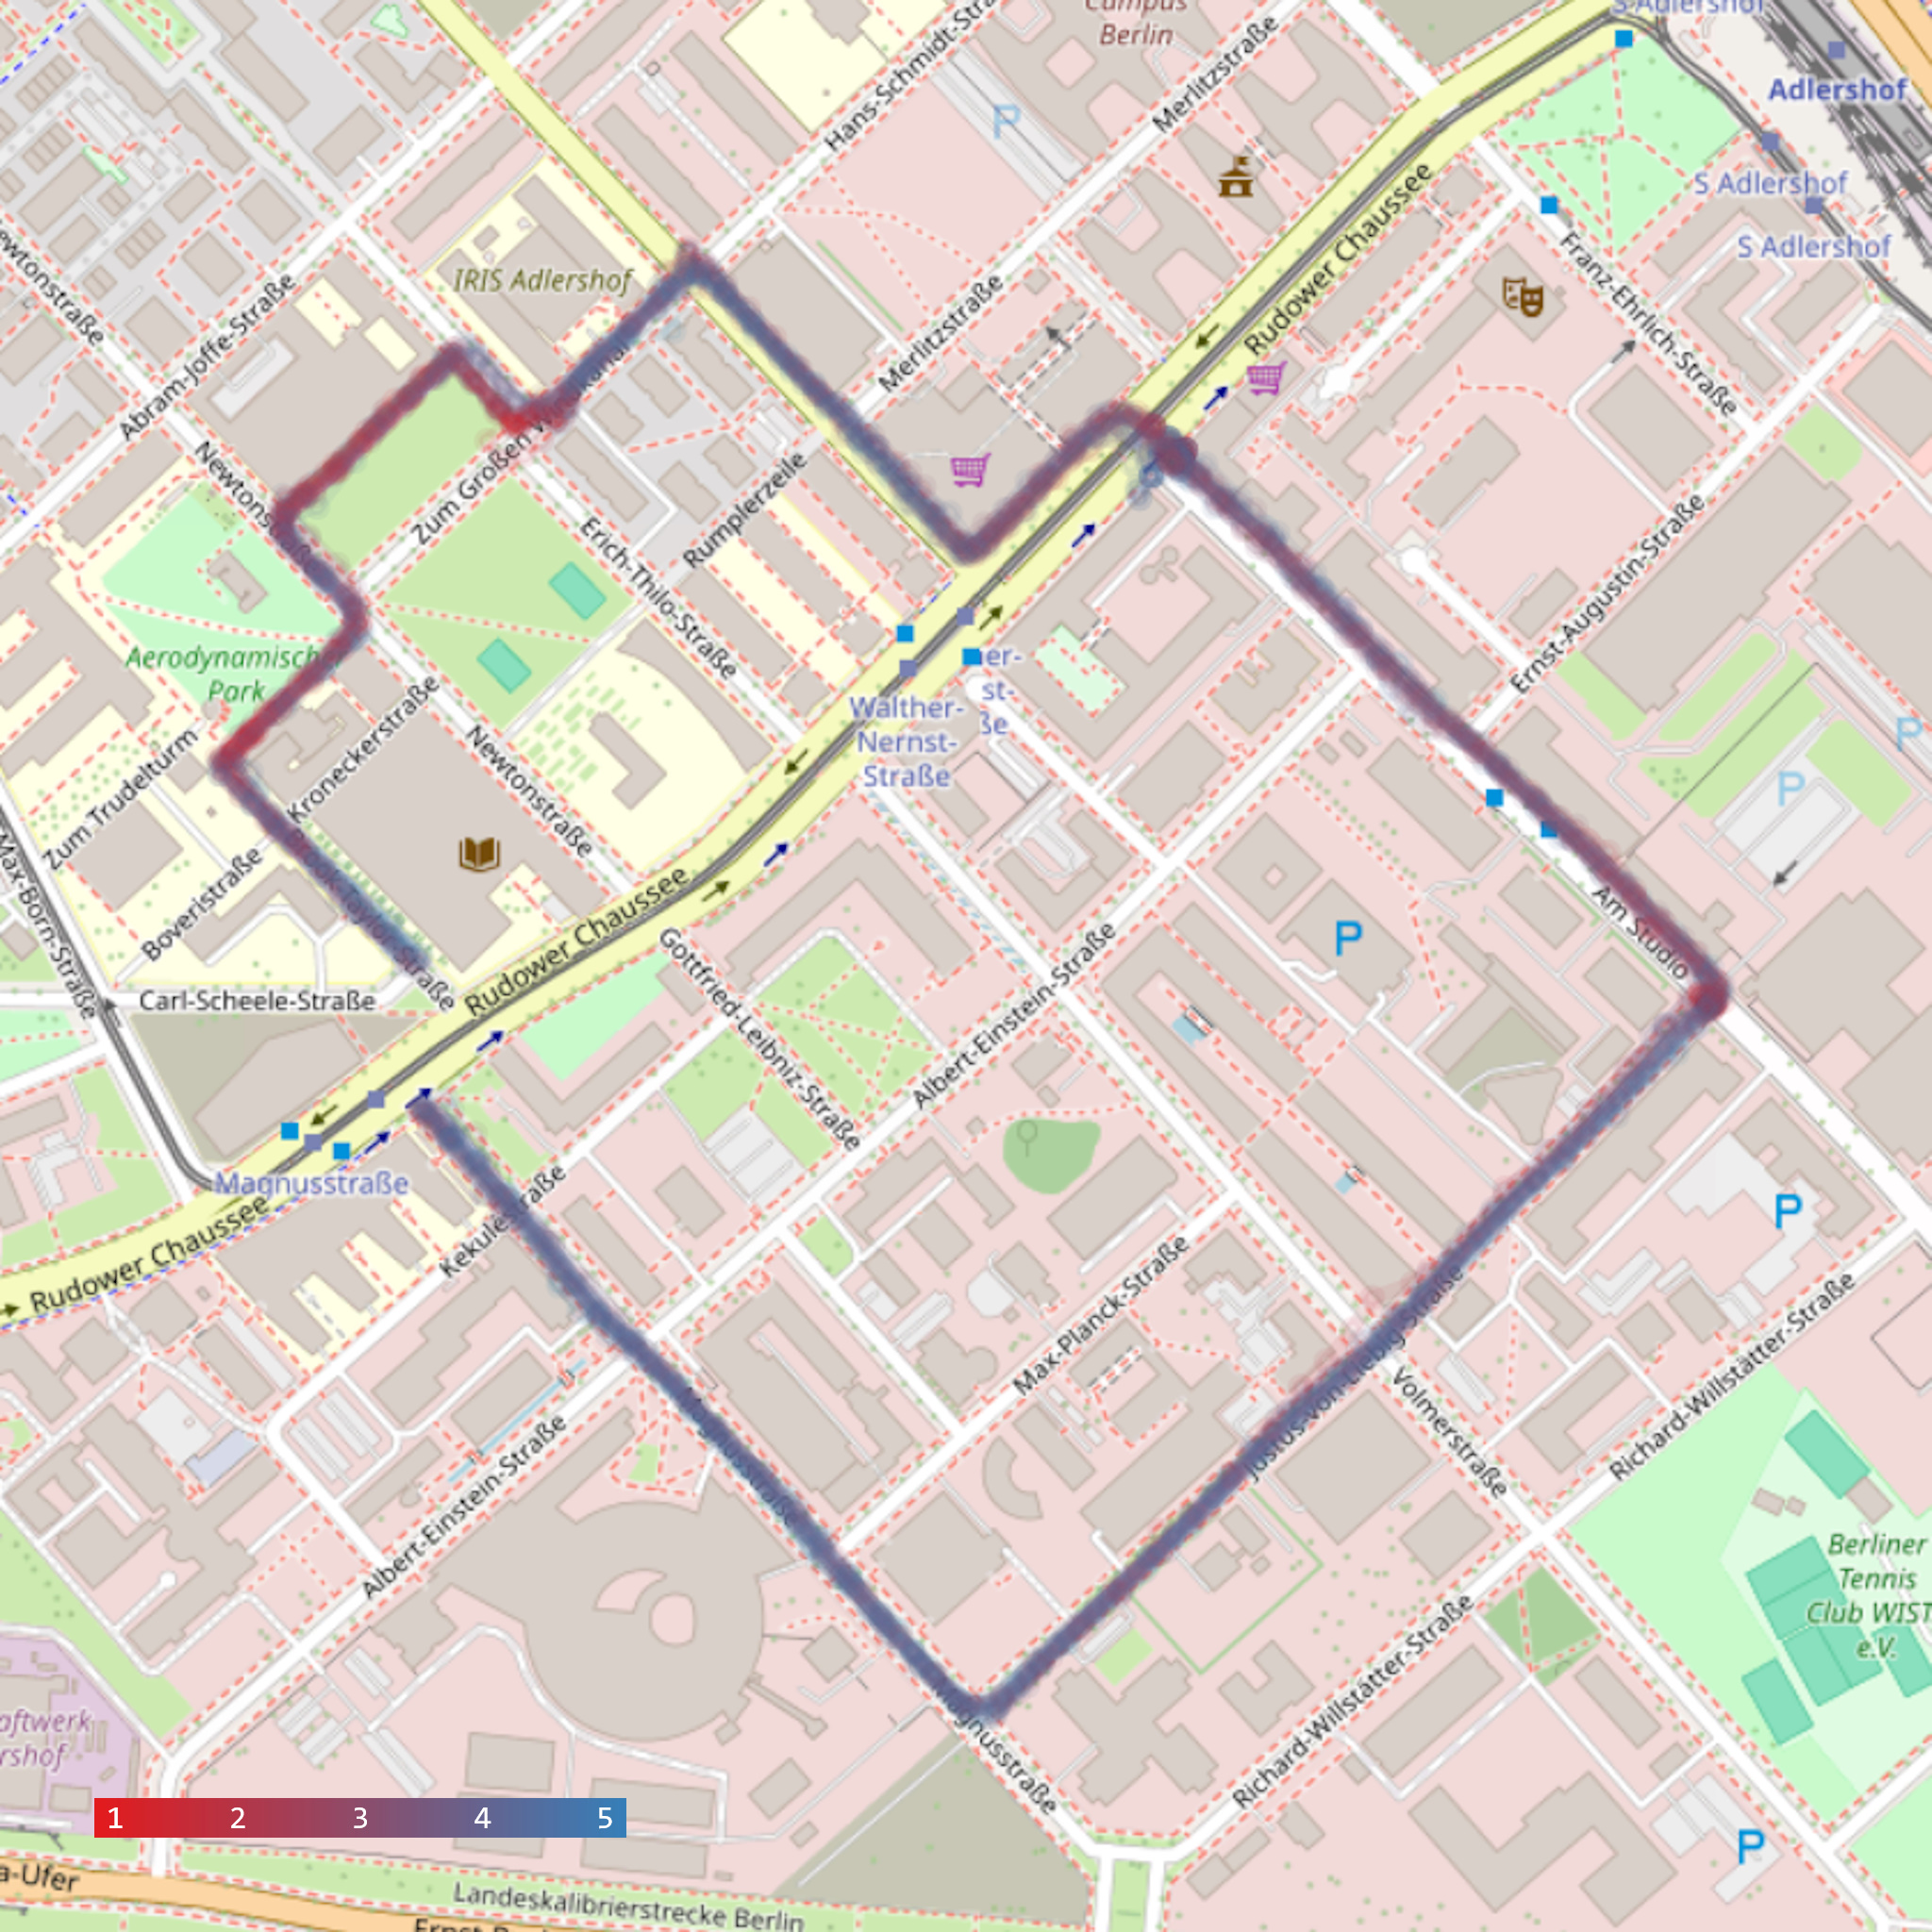
\includegraphics[width=.9\linewidth]{images/ratings_south_route.jpg}
        \caption{South route}
        \label{fig:ratings_south_route}
    \end{subfigure}\
    \caption{Combined ratings from all methods}
    \label{fig:route_ratings}
\end{figure}

\subsubsection{Preprocessing}\label{subsec:preprocessing}

Preprocessing of the recorded data was largely performed by hand, with the help of some simple python scripts.
The start and end position of all data recordings were adjusted manually, to remove unneeded data.
For the \audiorecording method, we had to manually listen to each audio file and extract the ratings performed by participants to match them to the recorded timestamps and GPS locations.
A similar process was used for the \mapping method to match the sections drawn on the paper maps to the recorded data.
Our \likertshift method required no further preprocessing.

\subsubsection{Evaluation}

As mentioned in \autoref{subsec:recording_methods}, comparing subjective data is inherently hard.
To perform our analysis, we categorized our original reference routes by road type and resampled them to $\sim\SI{1}{m}$ segments.
Then, we projected all recorded data from each method to them.
This left us with a combination of rating and road-type for each $\SI{1}{m}$ segment of each recording.
We then gathered all ratings by road-type for each method and computed their mean value, variance, and standard deviation, to see if we could see any drastic differences (see \autoref{table:likertshift_eval}).

\begin{table}[!htb]
    \footnotesize
    \centering
    \begin{tabular}{l|ccccccc}
        \multirow{2}{*}{\likertshift} & \multicolumn{7}{c}{Road Type}\\
        \cline{2-8}
        &&&&&&&\\[-1em]
        & Road & Bike Path & Mixed Path & Pedestrian Way & Wood Path & Field & Lawn\\[0.15em]
        \hline
        &&&&&&&\\[-0.8em]
        MEAN     & 3.7661 & 3.4624 & 3.7708 & 3.0176 & 1.8114 & 1.9804 & 2.8664\\[0.3em]
        VARIANCE & 0.9327 & 0.9140 & 0.8548 & 0.8873 & 0.9661 & 1.2512 & 1.3830\\[0.3em]
        STDDEV   & 0.9658 & 0.9560 & 0.9246 & 0.9420 & 0.9829 & 1.1186 & 1.1760\\
    \end{tabular}

    \vspace{1em}
    \begin{tabular}{l|ccccccc}
        \textsf{Audio} & \multicolumn{7}{c}{Road Type}\\
        \cline{2-8}
        &&&&&&&\\[-1em]
        \textsf{Recording} & Road & Bike Path & Mixed Path & Pedestrian Way & Wood Path & Field & Lawn\\[0.15em]
        \hline
        &&&&&&&\\[-0.8em]
        MEAN     & 3.6622 & 3.4978 & 3.7915 & 2.9559 & 2.5513 & 1.6895 & 2.4405\\[0.3em]
        VARIANCE & 0.8519 & 0.7970 & 0.8172 & 1.4158 & 0.5622 & 1.2402 & 0.9290\\[0.3em]
        STDDEV   & 0.9230 & 0.8927 & 0.9040 & 1.1899 & 0.7498 & 1.1137 & 0.9638\\
    \end{tabular}

    \vspace{1em}
    \begin{tabular}{l|ccccccc}
        \multirow{2}{*}{\mapping} & \multicolumn{7}{c}{Road Type}\\
        \cline{2-8}
        &&&&&&&\\[-1em]
        & Road & Bike Path & Mixed Path & Pedestrian Way & Wood Path & Field & Lawn\\[0.15em]
        \hline
        &&&&&&&\\[-0.8em]
        MEAN     & 3.7476 & 3.4952 & 3.7230 & 3.3553 & 2.3586 & 1.0000 & 3.0291\\[0.3em]
        VARIANCE & 0.9192 & 1.0542 & 1.0379 & 1.2773 & 1.5566 & 0.0000 & 1.0891\\[0.3em]
        STDDEV   & 0.9587 & 1.0267 & 1.0188 & 1.1302 & 1.2476 & 0.0000 & 1.0436\\
    \end{tabular}
    \caption{Evaluation of the recorded quantitative data}
    \label{table:likertshift_eval}
\end{table}

\subsection{Questionnaires and Interviews}

We evaluated each component of the \citetextnoref{nasa_tlx}{TLX} and \citetextnoref{ueq+}{UEQ+} surveys separately, without computing an overall index, because we are most interested in what components cause increased task load or affect the user experience.

The \textit{Physical Demand}, \textit{Temporal Demand}, and \textit{Performance} metrics of the \citetextnoref{nasa_tlx}{TLX} showed little statistical evidence for differences between methods.
The most notable difference is the increased \textit{Mental Demand} objected by the \mapping method, as well as higher \textit{Frustration} and perceived \textit{Effort} in comparison to the live-recording methods.
There is insufficient statistical evidence for differences in task load between our \likertshift method and the \audiorecording method.

\begin{figure}[!htb]
    \centering
    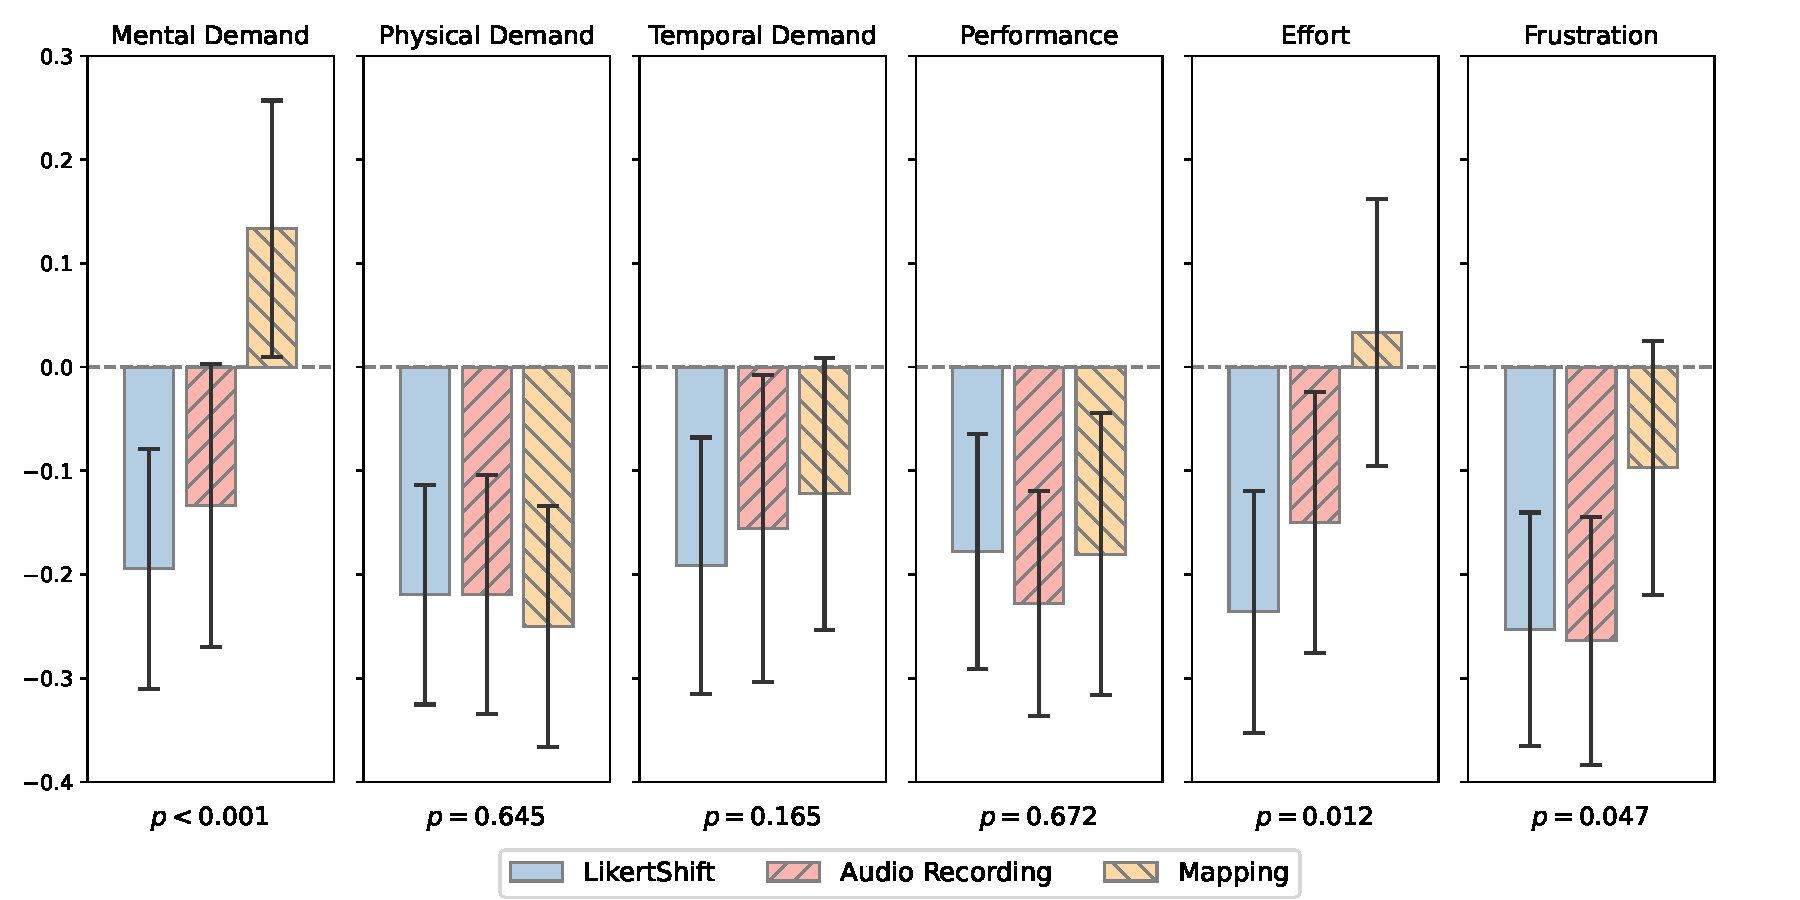
\includegraphics[height=0.5\linewidth]{../evaluation/eval_tlx.pdf}
    \caption{TLX results (the errorbars denote the confidence interval based on a student's distribution; $p$ values are computed using a Friedman test; values are normalized from -1 to 1)}
    \label{fig:eval_tlx}
\end{figure}

\bigbreak\noindent
The evaluation of the \citetextnoref{ueq+}{UEQ+} metrics turned out to be more interesting.
We observed incredibly evidence for the \textit{Attractiveness} and \textit{Intuitiveness} of our \likertshift method, compared to the other ones.
While participants perceived the \likertshift and \audiorecording methods to be similarly \textit{Efficient}, in comparison, the \mapping method was perceived as highly inefficient.
We can also observe low \textit{Social Acceptance} ratings of the \audiorecording method.

These findings were confirmed by our performed interviews.
Multiple participants denoted that the additional time requirements of the \mapping method make using it very unattractive to them.
Similarly, the majority of participants stated they did not like to talk during cycling and found it “awkward” to perform the \audiorecording method.
When asked what method participants would choose to conduct a longer ($\sim\SI{2}{weeks}$) field-study which would require them to record their travel satisfaction on all of their commutes and other trips, 17 out of 18 participants chose our \likertshift method.

\begin{figure}[!htb]
    \centering
    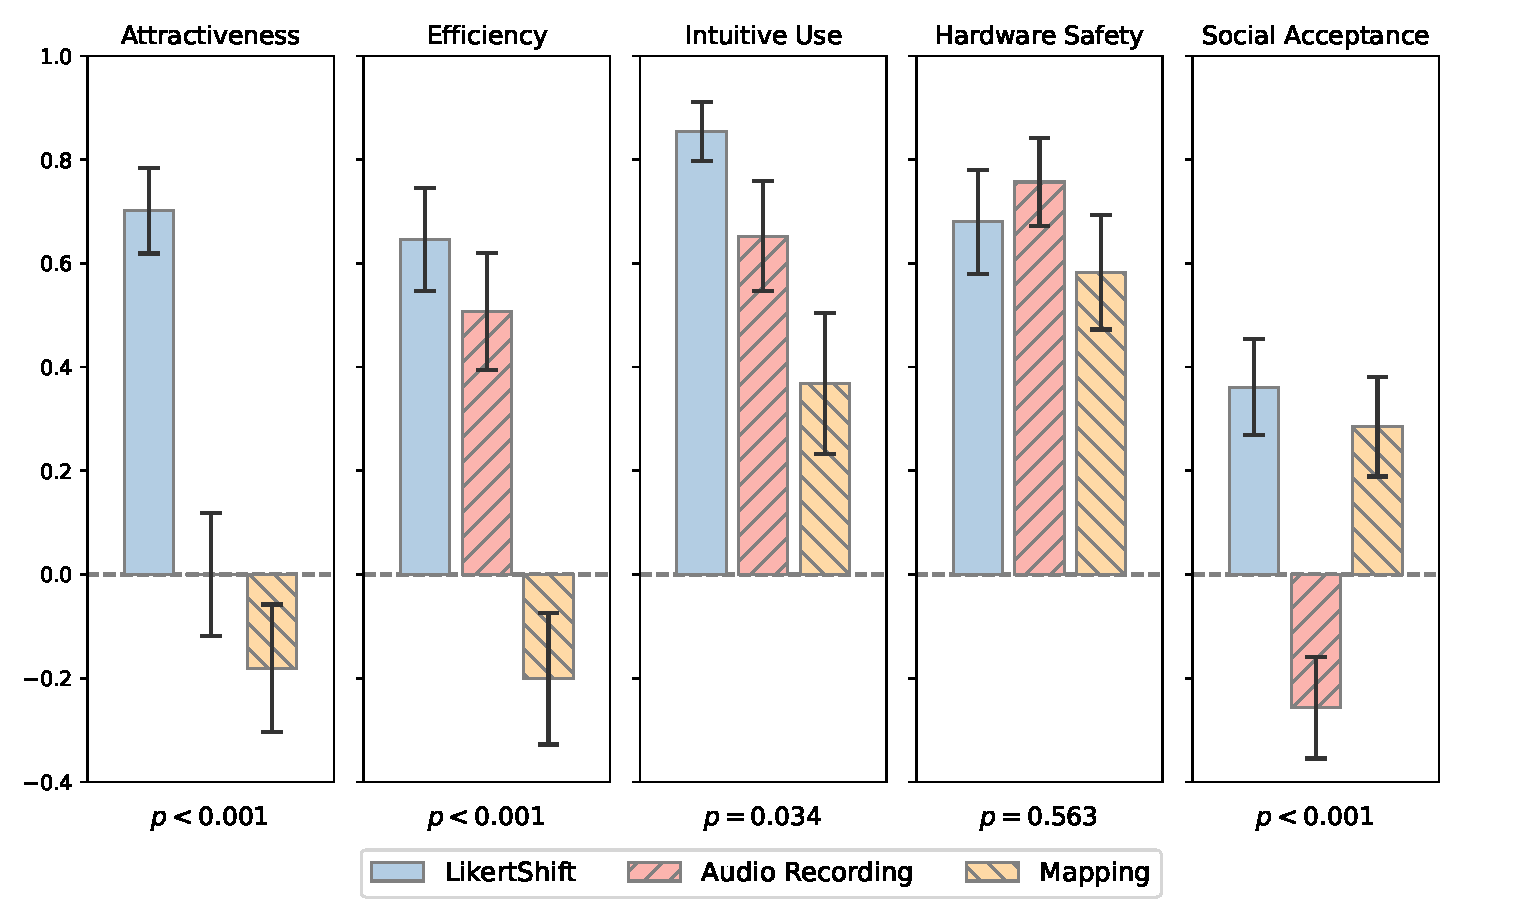
\includegraphics[height=0.5\linewidth]{../evaluation/eval_ueq.pdf}
    \caption{UEQ+ results (the errorbars denote the confidence interval based on a student's distribution; $p$ values are computed using a Friedman test; values are normalized from -1 to 1)}
    \label{fig:eval_ueq}
\end{figure}

\newpage\section{Discussion}\label{sec:discussion}

\subsection{Research Questions}

\subsection{Design Requirements}\label{subsec:discussion_design_requirements}

\subsection{Future Work}

\begin{itemize}
    \item hybrid methods (manual mapping)
    \item missing software qol features
    \item longer studies
\end{itemize}

\newpage\section{Conclusion}\label{sec:conclusion}

In this work, we described the successful design and construction of the \likertshift, a prototype device that can be used to record cyclists' subjective experiences, as well as its evaluation against other state-of-the-art methods in a semi-naturalistic field-study.
Although quantitative analysis of recorded data revealed little to no statistical evidence supporting a measurable improvement in data quality using our developed \likertshift method, qualitative assessments of participants' opinions regarding the different methods provided valuable insights.
They highlighted the perceived attractiveness, intuitiveness, and efficiency of using our physical device.
Participants also voiced concerns about the social acceptance of speech recording during cycling and the high effort and increased mental demand associated with retrospective mental mapping approaches that rely on the memorization of route segments, particularly for longer routes.
From our collected evidence, we see great potential in using physical devices for recording data on cyclists' subjective experiences, especially in longer, more naturalistic field-studies.


%%%%%%%%%%%%%%%%%%%%%%%%%%%%%%%%%%%_BIBLIOGRAPHY_%%%%%%%%%%%%%%%%%%%%%%%%%%%%%%%%%%%
% create your bibliography based on your files in library/...
% remember to edit \addbibresource in the TEMPLATE_PACKAGSES area above!
\newpage
\pagenumbering{roman} % start roman page numbers from here (optional)
\bibliographystyle{abbrvurl}
\bibliography{references.bib}
%%%%%%%%%%%%%%%%%%%%%%%%%%%%%%%%%%%%%_APPENDIX_%%%%%%%%%%%%%%%%%%%%%%%%%%%%%%%%%%%%
\section*{Appendix} \label{Appendix}
\addcontentsline{toc}{section}{Appendix}    % adds entry to table of contents
\selbstaendigkeitserklaerung{\today}
%\input{chapters/xxx}                       % add in case you have additional images/tables
\end{document}
%%%%%%%%%%%%%%%%%%%%%%%%%%%%%%%%%%%%%%%%%%%%%%%%%%%%%%%%%%%%%%%%%%%%%%%%%%%%%%%%%%%%
